\pdfoutput=1
%% luca_template150501.tex --- 
%% 
%% Author: PGL  Porta Mana
%% Created: 2015-05-01T20:53:34+0200
%% Last-Updated: 2017-07-02T00:39:19+0200
%%%%%%%%%%%%%%%%%%%%%%%%%%%%%%%%%%%%%%%%%%%%%%%%%%%%%%%%%%%%%%%%%%%%%%
%Report-no: ***
\newif\ifafour
\afourtrue % true = A4, false = A5
\newif\iftypodisclaim % typographical disclaim on the side
\typodisclaimfalse
\newcommand*{\memfontfamily}{zplx}
\newcommand*{\memfontpack}{newpxtext}
\documentclass[\ifafour a4paper,12pt,\else a5paper,10pt,\fi%extrafontsizes,%
onecolumn,oneside,article,%french,italian,german,swedish,latin,
british%
]{memoir}
\newif\ifpublic
\publictrue % true = for publication, false = personal notes
\newcommand*{\firstdraft}{27 November 2016}
\newcommand*{\oggi}{\today}
\newcommand*{\propertitle}{Inferring health conditions from fMRI-graph data}
\newcommand*{\pdftitle}{Inferring health conditions from fMRI-graph data}
\newcommand*{\headtitle}{\pdftitle}
\newcommand*{\pdfauthor}{P.G.L.  Porta Mana, C. Bachmann, A. Morrison}
\newcommand*{\headauthor}{Bachmann, Porta Mana, Morrison}
\newcommand*{\reporthead}{}

%%%%%%%%%%%%%%%%%%%%%%%%%%%%%%%%%%%%%%%%%%%%%%%%%%%%%%%%%%%%%%%%%%%%%%%%%%%%
%%%%%%%%%%%%%%%%%%%%%%%%%%%%%%%%%%%%%%%%%%%%%%%%%%%%%%%%%%%%%%%%%%%%%%%%%%%%
%\usepackage{pifont}
%\usepackage{fontawesome}
\usepackage[T1]{fontenc} 
\input{glyphtounicode} \pdfgentounicode=1
\usepackage[utf8]{inputenx}
%\usepackage{newunicodechar}
% \newunicodechar{Ĕ}{\u{E}}
% \newunicodechar{ĕ}{\u{e}}
% \newunicodechar{Ĭ}{\u{I}}
% \newunicodechar{ĭ}{\u{\i}}
% \newunicodechar{Ŏ}{\u{O}}
% \newunicodechar{ŏ}{\u{o}}
% \newunicodechar{Ŭ}{\u{U}}
% \newunicodechar{ŭ}{\u{u}}
% \newunicodechar{Ā}{\=A}
% \newunicodechar{ā}{\=a}
% \newunicodechar{Ē}{\=E}
% \newunicodechar{ē}{\=e}
% \newunicodechar{Ī}{\=I}
% \newunicodechar{ī}{\={\i}}
% \newunicodechar{Ō}{\=O}
% \newunicodechar{ō}{\=o}
% \newunicodechar{Ū}{\=U}
% \newunicodechar{ū}{\=u}
% \newunicodechar{Ȳ}{\=Y}
% \newunicodechar{ȳ}{\=y}

%\newcommand*{\bmmax}{0} % reduce number of bold fonts, before bm
\newcommand*{\hmmax}{0} % reduce number of heavy fonts, before bm
\usepackage{textcomp}
\usepackage[normalem]{ulem}
% \makeatletter
% \def\ssout{\bgroup \ULdepth=-.35ex%\UL@setULdepth
%  \markoverwith{\lower\ULdepth\hbox
%    {\kern-.03em\vbox{\hrule width.2em\kern1.2\p@\hrule}\kern-.03em}}%
%  \ULon}
% \makeatother
\usepackage{amsmath}
\usepackage{mathtools}
\usepackage{empheq}% automatically calls amsmath and mathtools
\newcommand*{\widefbox}[1]{\fbox{\hspace{1em}#1\hspace{1em}}}
\setlength{\multlinegap}{0pt}
%\usepackage{fancybox}
\usepackage{framed}
% \usepackage[misc]{ifsym} % for dice
% \newcommand*{\diceone}{{\scriptsize\Cube{1}}}
\usepackage{amssymb}
\usepackage{amsxtra}

\usepackage[main=british,french,italian,german,swedish,latin,esperanto]{babel}\selectlanguage{british}
\newcommand*{\langfrench}{\foreignlanguage{french}}
\newcommand*{\langgerman}{\foreignlanguage{german}}
\newcommand*{\langitalian}{\foreignlanguage{italian}}
\newcommand*{\langswedish}{\foreignlanguage{swedish}}
\newcommand*{\langlatin}{\foreignlanguage{latin}}
\newcommand*{\langnohyph}{\foreignlanguage{nohyphenation}}

\usepackage[autostyle=false,autopunct=false,english=british]{csquotes}
\setquotestyle{american}

\usepackage{amsthm}
\newcommand*{\QED}{\textsc{q.e.d.}}
\renewcommand*{\qedsymbol}{\QED}
\theoremstyle{remark}
\newtheorem{note}{Note}
\newtheorem*{remark}{Note}
\newtheoremstyle{innote}{\parsep}{\parsep}{\footnotesize}{}{}{}{0pt}{}
\theoremstyle{innote}
\newtheorem*{innote}{}


\usepackage[shortlabels,inline]{enumitem}
\SetEnumitemKey{para}{itemindent=\parindent,leftmargin=0pt,listparindent=\parindent,parsep=0pt,itemsep=\topsep}
% \begin{asparaenum} = \begin{enumerate}[para]
% \begin{inparaenum} = \begin{enumerate*}
\setlist[enumerate,2]{label=\alph*.}
\setlist[enumerate]{leftmargin=\parindent}
\setlist[itemize]{leftmargin=\parindent}
\setlist[description]{leftmargin=\parindent}

\usepackage[babel,theoremfont]{newpxtext}
\usepackage[bigdelims,nosymbolsc%,smallerops % probably arXiv doesn't have it
]{newpxmath}
\useosf\linespread{1.083}
%% smaller operators for old version of newpxmath
\makeatletter
\def\re@DeclareMathSymbol#1#2#3#4{%
    \let#1=\undefined
    \DeclareMathSymbol{#1}{#2}{#3}{#4}}
%\re@DeclareMathSymbol{\bigsqcupop}{\mathop}{largesymbols}{"46}
%\re@DeclareMathSymbol{\bigodotop}{\mathop}{largesymbols}{"4A}
\re@DeclareMathSymbol{\bigoplusop}{\mathop}{largesymbols}{"4C}
\re@DeclareMathSymbol{\bigotimesop}{\mathop}{largesymbols}{"4E}
\re@DeclareMathSymbol{\sumop}{\mathop}{largesymbols}{"50}
\re@DeclareMathSymbol{\prodop}{\mathop}{largesymbols}{"51}
\re@DeclareMathSymbol{\bigcupop}{\mathop}{largesymbols}{"53}
\re@DeclareMathSymbol{\bigcapop}{\mathop}{largesymbols}{"54}
%\re@DeclareMathSymbol{\biguplusop}{\mathop}{largesymbols}{"55}
\re@DeclareMathSymbol{\bigwedgeop}{\mathop}{largesymbols}{"56}
\re@DeclareMathSymbol{\bigveeop}{\mathop}{largesymbols}{"57}
%\re@DeclareMathSymbol{\bigcupdotop}{\mathop}{largesymbols}{"DF}
%\re@DeclareMathSymbol{\bigcapplusop}{\mathop}{largesymbolsPXA}{"00}
%\re@DeclareMathSymbol{\bigsqcupplusop}{\mathop}{largesymbolsPXA}{"02}
%\re@DeclareMathSymbol{\bigsqcapplusop}{\mathop}{largesymbolsPXA}{"04}
%\re@DeclareMathSymbol{\bigsqcapop}{\mathop}{largesymbolsPXA}{"06}
\re@DeclareMathSymbol{\bigtimesop}{\mathop}{largesymbolsPXA}{"10}
%\re@DeclareMathSymbol{\coprodop}{\mathop}{largesymbols}{"60}
%\re@DeclareMathSymbol{\varprod}{\mathop}{largesymbolsPXA}{16}
\makeatother


%% With euler font cursive for Greek letters - the [1] means 100% scaling
\DeclareFontFamily{U}{egreek}{\skewchar\font'177}%
\DeclareFontShape{U}{egreek}{m}{n}{<-6>s*[1]eurm5 <6-8>s*[1]eurm7 <8->s*[1]eurm10}{}%
\DeclareFontShape{U}{egreek}{m}{it}{<->s*[1]eurmo10}{}%
\DeclareFontShape{U}{egreek}{b}{n}{<-6>s*[1]eurb5 <6-8>s*[1]eurb7 <8->s*[1]eurb10}{}%
\DeclareFontShape{U}{egreek}{b}{it}{<->s*[1]eurbo10}{}%
\DeclareSymbolFont{egreeki}{U}{egreek}{m}{it}%
\SetSymbolFont{egreeki}{bold}{U}{egreek}{b}{it}% from the amsfonts package
\DeclareSymbolFont{egreekr}{U}{egreek}{m}{n}%
\SetSymbolFont{egreekr}{bold}{U}{egreek}{b}{n}% from the amsfonts package
% Take also \sum, \prod, \coprod symbols from Euler fonts
\DeclareFontFamily{U}{egreekx}{\skewchar\font'177}
\DeclareFontShape{U}{egreekx}{m}{n}{%
       <-7.5>s*[0.9]euex7%
    <7.5-8.5>s*[0.9]euex8%
    <8.5-9.5>s*[0.9]euex9%
    <9.5->s*[0.9]euex10%
}{}
\DeclareSymbolFont{egreekx}{U}{egreekx}{m}{n}
\DeclareMathSymbol{\sumop}{\mathop}{egreekx}{"50}
\DeclareMathSymbol{\prodop}{\mathop}{egreekx}{"51}
\DeclareMathSymbol{\coprodop}{\mathop}{egreekx}{"60}
\makeatletter
\def\sum{\DOTSI\sumop\slimits@}
\def\prod{\DOTSI\prodop\slimits@}
\def\coprod{\DOTSI\coprodop\slimits@}
\makeatother
\let\varpartial\undefined
\let\partialup\undefined
\let\alpha\undefined
\let\beta\undefined
\let\gamma\undefined
\let\delta\undefined
\let\epsilon\undefined
\let\zeta\undefined
\let\eta\undefined
\let\theta\undefined
\let\iota\undefined
\let\kappa\undefined
\let\lambda\undefined
\let\mu\undefined
\let\nu\undefined
\let\xi\undefined
\let\omicron\undefined
\let\pi\undefined
\let\rho\undefined
\let\sigma\undefined
\let\tau\undefined
\let\upsilon\undefined
\let\phi\undefined
\let\chi\undefined
\let\psi\undefined
\let\omega\undefined
\let\varepsilon\undefined
\let\vartheta\undefined
\let\varpi\undefined
\let\varrho\undefined 
\let\varsigma\undefined
\let\varkappa\undefined
\let\varphi\undefined
%
\let\varAlpha\undefined
\let\varBeta\undefined
\let\varGamma\undefined
\let\varDelta\undefined
\let\varEpsilon\undefined
\let\varZeta\undefined
\let\varEta\undefined
\let\varTheta\undefined
\let\varIota\undefined
\let\varKappa\undefined
\let\varLambda\undefined
\let\varMu\undefined
\let\varNu\undefined
\let\varXi\undefined
\let\varOmicron\undefined
\let\varPi\undefined
\let\varRho\undefined
\let\varSigma\undefined
\let\varTau\undefined
\let\varUpsilon\undefined
\let\varPhi\undefined
\let\varChi\undefined
\let\varPsi\undefined
\let\varOmega\undefined
%
\let\Alpha\undefined
\let\Beta\undefined
\let\Gamma\undefined
\let\Delta\undefined
\let\Epsilon\undefined
\let\Zeta\undefined
\let\Eta\undefined
\let\Theta\undefined
\let\Iota\undefined
\let\Kappa\undefined
\let\Lambda\undefined
\let\Mu\undefined
\let\Nu\undefined
\let\Xi\undefined
\let\Omicron\undefined
\let\Pi\undefined
\let\Rho\undefined
\let\Sigma\undefined
\let\Tau\undefined
\let\Upsilon\undefined
\let\Phi\undefined
\let\Chi\undefined
\let\Psi\undefined
\let\Omega\undefined
%
\let\alphaup\undefined
\let\betaup\undefined
\let\gammaup\undefined
\let\deltaup\undefined
\let\epsilonup\undefined
\let\zetaup\undefined
\let\etaup\undefined
\let\thetaup\undefined
\let\iotaup\undefined
\let\kappaup\undefined
\let\lambdaup\undefined
\let\muup\undefined
\let\nuup\undefined
\let\xiup\undefined
\let\omicronup\undefined
\let\piup\undefined
\let\rhoup\undefined
\let\sigmaup\undefined
\let\tauup\undefined
\let\upsilonup\undefined
\let\phiup\undefined
\let\chiup\undefined
\let\psiup\undefined
\let\omegaup\undefined
\let\varepsilonup\undefined
\let\varthetaup\undefined
\let\varpiup\undefined
\let\varrhoup\undefined
\let\varsigmaup\undefined
\let\varkappaup\undefined
\let\varphiup\undefined
 % to make sure no CMF greek letters sneak in
% Greek letters not usually given in LaTeX. Comment the unneeded ones
% \DeclareMathSymbol{\varpartial}{\mathalpha}{egreeki}{"40}
 \DeclareMathSymbol{\partialup}{\mathalpha}{egreekr}{"40}
% \DeclareMathSymbol{\alpha}{\mathalpha}{egreeki}{"0B}
% \DeclareMathSymbol{\beta}{\mathalpha}{egreeki}{"0C}
% \DeclareMathSymbol{\gamma}{\mathalpha}{egreeki}{"0D}
% \DeclareMathSymbol{\delta}{\mathalpha}{egreeki}{"0E}
 \DeclareMathSymbol{\epsilon}{\mathalpha}{egreeki}{"0F}
% \DeclareMathSymbol{\zeta}{\mathalpha}{egreeki}{"10}
% \DeclareMathSymbol{\eta}{\mathalpha}{egreeki}{"11}
% \DeclareMathSymbol{\theta}{\mathalpha}{egreeki}{"12}
% \DeclareMathSymbol{\iota}{\mathalpha}{egreeki}{"13}
 \DeclareMathSymbol{\kappa}{\mathalpha}{egreeki}{"14}
 \DeclareMathSymbol{\lambda}{\mathalpha}{egreeki}{"15}
 \DeclareMathSymbol{\mu}{\mathalpha}{egreeki}{"16}
 \DeclareMathSymbol{\nu}{\mathalpha}{egreeki}{"17}
% \DeclareMathSymbol{\xi}{\mathalpha}{egreeki}{"18}
% \DeclareMathSymbol{\omicron}{\mathalpha}{egreeki}{"6F}
% \DeclareMathSymbol{\pi}{\mathalpha}{egreeki}{"19}
% \DeclareMathSymbol{\rho}{\mathalpha}{egreeki}{"1A}
% \DeclareMathSymbol{\sigma}{\mathalpha}{egreeki}{"1B}
% \DeclareMathSymbol{\tau}{\mathalpha}{egreeki}{"1C}
% \DeclareMathSymbol{\upsilon}{\mathalpha}{egreeki}{"1D}
% \DeclareMathSymbol{\phi}{\mathalpha}{egreeki}{"1E}
% \DeclareMathSymbol{\chi}{\mathalpha}{egreeki}{"1F}
% \DeclareMathSymbol{\psi}{\mathalpha}{egreeki}{"20}
% \DeclareMathSymbol{\omega}{\mathalpha}{egreeki}{"21}
% \DeclareMathSymbol{\varepsilon}{\mathalpha}{egreeki}{"22}
% \DeclareMathSymbol{\vartheta}{\mathalpha}{egreeki}{"23}
% \DeclareMathSymbol{\varpi}{\mathalpha}{egreeki}{"24}
% \let\varrho\rho 
% \let\varsigma\sigma
 \let\varkappa\kappa
% \DeclareMathSymbol{\varphi}{\mathalpha}{egreeki}{"27}
% %
% \DeclareMathSymbol{\varAlpha}{\mathalpha}{egreeki}{"41}
% \DeclareMathSymbol{\varBeta}{\mathalpha}{egreeki}{"42}
% \DeclareMathSymbol{\varGamma}{\mathalpha}{egreeki}{"00}
 \DeclareMathSymbol{\varDelta}{\mathalpha}{egreeki}{"01}
 \DeclareMathSymbol{\varEpsilon}{\mathalpha}{egreeki}{"45}
% \DeclareMathSymbol{\varZeta}{\mathalpha}{egreeki}{"5A}
% \DeclareMathSymbol{\varEta}{\mathalpha}{egreeki}{"48}
% \DeclareMathSymbol{\varTheta}{\mathalpha}{egreeki}{"02}
 \DeclareMathSymbol{\varIota}{\mathalpha}{egreeki}{"49}
% \DeclareMathSymbol{\varKappa}{\mathalpha}{egreeki}{"4B}
% \DeclareMathSymbol{\varLambda}{\mathalpha}{egreeki}{"03}
% \DeclareMathSymbol{\varMu}{\mathalpha}{egreeki}{"4D}
% \DeclareMathSymbol{\varNu}{\mathalpha}{egreeki}{"4E}
% \DeclareMathSymbol{\varXi}{\mathalpha}{egreeki}{"04}
% \DeclareMathSymbol{\varOmicron}{\mathalpha}{egreeki}{"4F}
% \DeclareMathSymbol{\varPi}{\mathalpha}{egreeki}{"05}
% \DeclareMathSymbol{\varRho}{\mathalpha}{egreeki}{"50}
 \DeclareMathSymbol{\varSigma}{\mathalpha}{egreeki}{"06}
% \DeclareMathSymbol{\varTau}{\mathalpha}{egreeki}{"54}
% \DeclareMathSymbol{\varUpsilon}{\mathalpha}{egreeki}{"07}
% \DeclareMathSymbol{\varPhi}{\mathalpha}{egreeki}{"08}
 \DeclareMathSymbol{\varChi}{\mathalpha}{egreeki}{"58}
% \DeclareMathSymbol{\varPsi}{\mathalpha}{egreeki}{"09}
% \DeclareMathSymbol{\varOmega}{\mathalpha}{egreeki}{"0A} 
% %
% \DeclareMathSymbol{\Alpha}{\mathalpha}{egreekr}{"41}
% \DeclareMathSymbol{\Beta}{\mathalpha}{egreekr}{"42}
 \DeclareMathSymbol{\Gamma}{\mathalpha}{egreekr}{"00}
% \DeclareMathSymbol{\Delta}{\mathalpha}{egreekr}{"01}
% \DeclareMathSymbol{\Epsilon}{\mathalpha}{egreekr}{"45}
% \DeclareMathSymbol{\Zeta}{\mathalpha}{egreekr}{"5A}
% \DeclareMathSymbol{\Eta}{\mathalpha}{egreekr}{"48}
% \DeclareMathSymbol{\Theta}{\mathalpha}{egreekr}{"02}
% \DeclareMathSymbol{\Iota}{\mathalpha}{egreekr}{"49}
% \DeclareMathSymbol{\Kappa}{\mathalpha}{egreekr}{"4B}
% \DeclareMathSymbol{\Lambda}{\mathalpha}{egreekr}{"03}
% \DeclareMathSymbol{\Mu}{\mathalpha}{egreekr}{"4D}
% \DeclareMathSymbol{\Nu}{\mathalpha}{egreekr}{"4E}
% \DeclareMathSymbol{\Xi}{\mathalpha}{egreekr}{"04}
% \DeclareMathSymbol{\Omicron}{\mathalpha}{egreekr}{"4F}
% \DeclareMathSymbol{\Pi}{\mathalpha}{egreekr}{"05}
% \DeclareMathSymbol{\Rho}{\mathalpha}{egreekr}{"50}
% \DeclareMathSymbol{\Sigma}{\mathalpha}{egreekr}{"06}
% \DeclareMathSymbol{\Tau}{\mathalpha}{egreekr}{"54}
% \DeclareMathSymbol{\Upsilon}{\mathalpha}{egreekr}{"07}
% \DeclareMathSymbol{\Phi}{\mathalpha}{egreekr}{"08}
% \DeclareMathSymbol{\Chi}{\mathalpha}{egreekr}{"58}
% \DeclareMathSymbol{\Psi}{\mathalpha}{egreekr}{"09}
% \DeclareMathSymbol{\Omega}{\mathalpha}{egreekr}{"0A}
% %
% \DeclareMathSymbol{\alphaup}{\mathalpha}{egreekr}{"0B}
% \DeclareMathSymbol{\betaup}{\mathalpha}{egreekr}{"0C}
% \DeclareMathSymbol{\gammaup}{\mathalpha}{egreekr}{"0D}
 \DeclareMathSymbol{\deltaup}{\mathalpha}{egreekr}{"0E}
% \DeclareMathSymbol{\epsilonup}{\mathalpha}{egreekr}{"0F}
% \DeclareMathSymbol{\zetaup}{\mathalpha}{egreekr}{"10}
% \DeclareMathSymbol{\etaup}{\mathalpha}{egreekr}{"11}
% \DeclareMathSymbol{\thetaup}{\mathalpha}{egreekr}{"12}
% \DeclareMathSymbol{\iotaup}{\mathalpha}{egreekr}{"13}
% \DeclareMathSymbol{\kappaup}{\mathalpha}{egreekr}{"14}
% \DeclareMathSymbol{\lambdaup}{\mathalpha}{egreekr}{"15}
% \DeclareMathSymbol{\muup}{\mathalpha}{egreekr}{"16}
% \DeclareMathSymbol{\nuup}{\mathalpha}{egreekr}{"17}
% \DeclareMathSymbol{\xiup}{\mathalpha}{egreekr}{"18}
% \DeclareMathSymbol{\omicronup}{\mathalpha}{egreekr}{"6F}
  \DeclareMathSymbol{\piup}{\mathalpha}{egreekr}{"19}
% \DeclareMathSymbol{\rhoup}{\mathalpha}{egreekr}{"1A}
% \DeclareMathSymbol{\sigmaup}{\mathalpha}{egreekr}{"1B}
% \DeclareMathSymbol{\tauup}{\mathalpha}{egreekr}{"1C}
% \DeclareMathSymbol{\upsilonup}{\mathalpha}{egreekr}{"1D}
% \DeclareMathSymbol{\phiup}{\mathalpha}{egreekr}{"1E}
% \DeclareMathSymbol{\chiup}{\mathalpha}{egreekr}{"1F}
% \DeclareMathSymbol{\psiup}{\mathalpha}{egreekr}{"20}
% \DeclareMathSymbol{\omegaup}{\mathalpha}{egreekr}{"21}
% \DeclareMathSymbol{\varepsilonup}{\mathalpha}{egreekr}{"22}
% \DeclareMathSymbol{\varthetaup}{\mathalpha}{egreekr}{"23}
% \DeclareMathSymbol{\varpiup}{\mathalpha}{egreekr}{"24}
% \let\varrhoup\rhoup 
% \let\varsigmaup\sigmaup
% \let\varkappaup\kappaup
% \DeclareMathSymbol{\varphiup}{\mathalpha}{egreekr}{"27}

% Optima as sans-serif font
%\usepackage%[scaled=0.9]%
%{classico}
\renewcommand\sfdefault{uop}
\DeclareMathAlphabet{\mathsf}  {T1}{\sfdefault}{m}{sl}
\SetMathAlphabet{\mathsf}{bold}{T1}{\sfdefault}{b}{sl}
\newcommand*{\mathte}[1]{\textbf{\textit{\textsf{#1}}}}
% Upright sans-serif math alphabet
% \DeclareMathAlphabet{\mathsu}  {T1}{\sfdefault}{m}{n}
% \SetMathAlphabet{\mathsu}{bold}{T1}{\sfdefault}{b}{n}

% DejaVu Mono as typewriter text
\usepackage[scaled=0.84]{DejaVuSansMono}


\usepackage{mathdots}

\usepackage[usenames]{xcolor}
% Tol (2012) colour-blind-, print-, screen-friendly colours; Munsell terminology
\definecolor{mybluishpurple}{RGB}{51,34,136}
\definecolor{myblue}{RGB}{136,204,238}
\definecolor{mybluishgreen}{RGB}{68,170,153}
\definecolor{mygreen}{RGB}{17,119,51}
\definecolor{mygreenishyellow}{RGB}{153,153,51}
\definecolor{myyellow}{RGB}{221,204,119}
\definecolor{myred}{RGB}{204,102,119}
\definecolor{mypurplishred}{RGB}{136,34,85}
\definecolor{myreddishpurple}{RGB}{170,68,153}
\definecolor{mygrey}{RGB}{221,221,221}
%\newcommand*\mycolourbox[1]{%
%\colorbox{mygrey}{\hspace{1em}#1\hspace{1em}}}
\colorlet{shadecolor}{mygrey}

\usepackage{bm}
\usepackage{microtype}

\usepackage[backend=biber,mcite,%subentry,
citestyle=authoryear-comp,bibstyle=pglpm-authoryear,autopunct=false,sorting=ny,sortcites=false,natbib=false,maxcitenames=1,maxbibnames=8,minbibnames=8,giveninits=true,uniquename=false,uniquelist=false,maxalphanames=1,block=space,hyperref=true,defernumbers=false,useprefix=true,sortupper=false,language=british,parentracker=false]{biblatex}
\DeclareSortingScheme{ny}{\sort{\field{sortname}\field{author}\field{editor}}\sort{\field{year}}}
\iffalse\makeatletter%%% replace parenthesis with brackets
\newrobustcmd*{\parentexttrack}[1]{%
  \begingroup
  \blx@blxinit
  \blx@setsfcodes
  \blx@bibopenparen#1\blx@bibcloseparen
  \endgroup}
\AtEveryCite{%
  \let\parentext=\parentexttrack%
  \let\bibopenparen=\bibopenbracket%
  \let\bibcloseparen=\bibclosebracket}
\makeatother\fi

\renewcommand*{\finalnamedelim}{, }
\setcounter{biburlnumpenalty}{1}
\setcounter{biburlucpenalty}{0}
\setcounter{biburllcpenalty}{1}
\DeclareDelimFormat{multicitedelim}{\addsemicolon\space}
\DeclareDelimFormat{compcitedelim}{\addsemicolon\space}
\DeclareDelimFormat{postnotedelim}{\space}
\addbibresource{portamanabib.bib}
\renewcommand{\bibfont}{\footnotesize}
%\appto{\citesetup}{\footnotesize}% smaller font for citations
\defbibheading{bibliography}[\bibname]{\section*{#1}\addcontentsline{toc}{section}{#1}%\markboth{#1}{#1}
}
\newcommand*{\citep}{\parencites}
\newcommand*{\citey}{\parencites*}
%\renewcommand*{\cite}{\parencite}
\renewcommand*{\cites}{\parencites}
\providecommand{\href}[2]{#2}
\providecommand{\eprint}[2]{\texttt{\href{#1}{#2}}}
\newcommand*{\amp}{\&}
% \newcommand*{\citein}[2][]{\textnormal{\textcite[#1]{#2}}%\addtocategory{extras}{#2}
% }
\newcommand*{\citein}[2][]{\textnormal{\citep[#1]{#2}}%\addtocategory{extras}{#2}
}
\newcommand*{\citebi}[2][]{\parencite[#1]{#2}%\addtocategory{extras}{#2}
}
\newcommand*{\subtitleproc}[1]{}
\newcommand*{\chapb}{ch.}

% \def\arxivp{}
% \def\mparcp{}
% \def\philscip{}
% \def\biorxivp{}
% \newcommand*{\arxivsi}{\texttt{arXiv} eprints available at \url{http://arxiv.org/}.\\}
% \newcommand*{\mparcsi}{\texttt{mp\_arc} eprints available at \url{http://www.ma.utexas.edu/mp_arc/}.\\}
% \newcommand*{\philscisi}{\texttt{philsci} eprints available at \url{http://philsci-archive.pitt.edu/}.\\}
% \newcommand*{\biorxivsi}{\texttt{bioRxiv} eprints available at \url{http://biorxiv.org/}.\\}
\newcommand*{\arxiveprint}[1]{%\global\def\arxivp{\arxivsi}%\citeauthor{0arxivcite}\addtocategory{ifarchcit}{0arxivcite}%eprint
\texttt{\urlalt{https://arxiv.org/abs/#1}{arXiv:\hspace{0pt}#1}}%
%\texttt{\href{http://arxiv.org/abs/#1}{\protect\url{arXiv:#1}}}%
%\renewcommand{\arxivnote}{\texttt{arXiv} eprints available at \url{http://arxiv.org/}.}
}
\newcommand*{\mparceprint}[1]{%\global\def\mparcp{\mparcsi}%\citeauthor{0mparccite}\addtocategory{ifarchcit}{0mparccite}%eprint
\texttt{\urlalt{http://www.ma.utexas.edu/mp_arc-bin/mpa?yn=#1}{mp\_arc:\hspace{0pt}#1}}%
%\texttt{\href{http://www.ma.utexas.edu/mp_arc-bin/mpa?yn=#1}{\protect\url{mp_arc:#1}}}%
%\providecommand{\mparcnote}{\texttt{mp_arc} eprints available at \url{http://www.ma.utexas.edu/mp_arc/}.}
}
\newcommand*{\philscieprint}[1]{%\global\def\philscip{\philscisi}%\citeauthor{0philscicite}\addtocategory{ifarchcit}{0philscicite}%eprint
\texttt{\urlalt{http://philsci-archive.pitt.edu/archive/#1}{PhilSci:\hspace{0pt}#1}}%
%\texttt{\href{http://philsci-archive.pitt.edu/archive/#1}{\protect\url{PhilSci:#1}}}%
%\providecommand{\mparcnote}{\texttt{philsci} eprints available at \url{http://philsci-archive.pitt.edu/}.}
}
\newcommand*{\biorxiveprint}[1]{%\global\def\biorxivp{\biorxivsi}%\citeauthor{0arxivcite}\addtocategory{ifarchcit}{0arxivcite}%eprint
\texttt{\urlalt{http://biorxiv.org/content/early/#1}{bioRxiv:\hspace{0pt}#1}}%
%\texttt{\href{http://arxiv.org/abs/#1}{\protect\url{arXiv:#1}}}%
%\renewcommand{\arxivnote}{\texttt{arXiv} eprints available at \url{http://arxiv.org/}.}
}
\newcommand*{\osfeprint}[1]{%
\texttt{\urlalt{https://osf.io/#1}{osf.io/#1}}%
}

\usepackage{graphicx}
\usepackage{wrapfig}

\usepackage{hyperref}
\usepackage[depth=4]{bookmark}
\hypersetup{colorlinks=true,bookmarksnumbered,pdfborder={0 0 0.25},citebordercolor={0.2 0.1333 0.5333},%bluish
citecolor=mybluishpurple,linkbordercolor={0.0667 0.4667 0.2},%greenish
linkcolor=mypurplishred,urlbordercolor={0.5333 0.1333 0.3333},%reddish
urlcolor=mygreen,breaklinks=true,pdftitle={\pdftitle},pdfauthor={\pdfauthor}}
% \usepackage[vertfit=local]{breakurl}% only for arXiv
\providecommand*{\urlalt}{\href}

%%% Layout. I do not know on which kind of paper the reader will print the
%%% paper on (A4? letter? one-sided? double-sided?). So I choose A5, which
%%% provides a good layout for reading on screen and save paper if printed
%%% two pages per sheet. Average length line is 66 characters and page
%%% numbers are centred.
\ifafour\setstocksize{297mm}{210mm}%{*}% A4
\else\setstocksize{210mm}{5.5in}%{*}% 210x139.7
\fi
\settrimmedsize{\stockheight}{\stockwidth}{*}
\setlxvchars[\normalfont] %313.3632pt for a 66-characters line
\setxlvchars[\normalfont]
\setlength{\trimtop}{0pt}
\setlength{\trimedge}{\stockwidth}
\addtolength{\trimedge}{-\paperwidth}
% The length of the normalsize alphabet is 133.05988pt - 10 pt = 26.1408pc
% The length of the normalsize alphabet is 159.6719pt - 12pt = 30.3586pc
% Bringhurst gives 32pc as boundary optimal with 69 ch per line
% The length of the normalsize alphabet is 191.60612pt - 14pt = 35.8634pc
\ifafour\settypeblocksize{*}{32pc}{1.618} % A4
%\setulmargins{*}{*}{1.667}%gives 5/3 margins % 2 or 1.667
\else\settypeblocksize{*}{26pc}{1.618}% nearer to a 66-line newpx and preserves GR
\fi
\setulmargins{*}{*}{1}%gives equal margins
\setlrmargins{*}{*}{*}
\setheadfoot{\onelineskip}{2.5\onelineskip}
\setheaderspaces{*}{2\onelineskip}{*}
\setmarginnotes{2ex}{10mm}{0pt}
\checkandfixthelayout[nearest]
\fixpdflayout
%%% End layout

%%% Sectioning
\newcommand*{\asudedication}[1]{%
{\par\centering\textit{#1}\par}}
\newenvironment{acknowledgements}{\section*{Thanks}\addcontentsline{toc}{section}{Thanks}}{\par}
\counterwithout{section}{chapter}
\setsecnumformat{\upshape\csname the#1\endcsname\quad}
\setsecheadstyle{\large\bfseries\sffamily%
\raggedright}
\setsubsecheadstyle{\bfseries\sffamily%
\raggedright}
%\setbeforesecskip{-1.5ex plus 1ex minus .2ex}% plus 1ex minus .2ex}
%\setaftersecskip{1.3ex plus .2ex }% plus 1ex minus .2ex}
%\setsubsubsecheadstyle{\bfseries\sffamily\slshape\raggedright}
%\setbeforesubsecskip{1.25ex plus 1ex minus .2ex }% plus 1ex minus .2ex}
\setaftersubsecskip{-1em}%{-0.5ex plus .2ex}% plus 1ex minus .2ex}
\setsubsecindent{0pt}%0ex plus 1ex minus .2ex}
\setparaheadstyle{\bfseries\sffamily%
\raggedright}
\setcounter{secnumdepth}{2}
\setlength{\headwidth}{\textwidth}
\newcommand{\addchap}[1]{\chapter*[#1]{#1}\addcontentsline{toc}{chapter}{#1}}
\newcommand{\addsec}[1]{\section*{#1}\addcontentsline{toc}{section}{#1}}
\newcommand{\addsubsec}[1]{\subsection*{#1}\addcontentsline{toc}{subsection}{#1}}
\newcommand{\addpara}[1]{\paragraph*{#1.}\addcontentsline{toc}{subsubsection}{#1}}
\newcommand{\addparap}[1]{\paragraph*{#1}\addcontentsline{toc}{subsubsection}{#1}}

% Headers and footers
\copypagestyle{manaart}{plain}
\makeheadrule{manaart}{\headwidth}{0.5\normalrulethickness}
\makeoddhead{manaart}{%
{\footnotesize\sffamily%
\scshape\headauthor}}{}{{\footnotesize\sffamily%
\headtitle}}
\makeoddfoot{manaart}{}{\thepage}{}
\newcommand*\autanet{\includegraphics[height=\heightof{M}]{autanet.pdf}}
\definecolor{mygray}{gray}{0.333}
\iftypodisclaim%
\ifafour\newcommand\addprintnote{\begin{picture}(0,0)%
\put(245,176){\makebox(0,0){\rotatebox{90}{\tiny\color{mygray}\textsf{This
            document is typographically designed for screen reading and
            two-up printing on A4 or Letter paper}}}}%
\end{picture}}% A4
\else\newcommand\addprintnote{\begin{picture}(0,0)%
\put(176,132){\makebox(0,0){\rotatebox{90}{\tiny\color{mygray}\textsf{This
            document is typographically designed for screen reading and
            two-up printing on A4 or Letter paper}}}}%
\end{picture}}\fi%afourtrue
\makeoddfoot{plain}{}{\makebox[0pt]{\thepage}\addprintnote}{}
\else
\makeoddfoot{plain}{}{\makebox[0pt]{\thepage}}{}
\fi%typodisclaimtrue
\makeoddhead{plain}{}{}{\footnotesize\reporthead}

\copypagestyle{manainitial}{plain}
\makeheadrule{manainitial}{\headwidth}{0.5\normalrulethickness}
\makeoddhead{manainitial}{%
\footnotesize\sffamily%
\scshape\headauthor}{}{\footnotesize\sffamily%
\headtitle}
\makeoddfoot{manaart}{}{\thepage}{}

\pagestyle{manaart}

\setlength{\droptitle}{-3.9\onelineskip}
\pretitle{\begin{center}\Large\sffamily%
\bfseries}
\posttitle{\bigskip\end{center}}

\makeatletter\newcommand*{\atf}{
\includegraphics[%trim=1pt 1pt 0pt 0pt,
totalheight=\heightof{@}]{atblack.png}}\makeatother
\providecommand{\affiliation}[1]{\textsl{\textsf{\footnotesize #1}}}
\providecommand{\epost}[1]{\texttt{\footnotesize\textless#1\textgreater}}
\providecommand{\email}[2]{\href{mailto:#1ZZ@#2 ((remove ZZ))}{#1\protect\atf#2}}

\preauthor{\vspace{-0.5\baselineskip}\begin{center}
\normalsize\sffamily%
\lineskip  0.5em}
\postauthor{\par\end{center}}
\predate{\DTMsetdatestyle{mydate}\begin{center}\footnotesize}
\postdate{\end{center}\vspace{-\medskipamount}}
\usepackage[british]{datetime2}
\DTMnewdatestyle{mydate}%
{% definitions
\renewcommand*{\DTMdisplaydate}[4]{%
\number##3\ \DTMenglishmonthname{##2} ##1}%
\renewcommand*{\DTMDisplaydate}{\DTMdisplaydate}%
}
\DTMsetdatestyle{mydate}


\setfloatadjustment{figure}{\footnotesize}
\captiondelim{\quad}
\captionnamefont{\footnotesize\sffamily%
}
\captiontitlefont{\footnotesize}
\firmlists*
\midsloppy

% handling orphan/widow lines:
\clubpenalty=10000
\widowpenalty=10000
\raggedbottom

\selectlanguage{british}\frenchspacing
%%%%%%%%%%%%%%%%%%%%%%%%%%%%%%%%%%%%%%%%%%%%%%%%%%%%%%%%%%%%%%%%%%%%%%%%%%%%
%%%%%%%%%%%%%%%%%%%%%%%%%%%%%%%%%%%%%%%%%%%%%%%%%%%%%%%%%%%%%%%%%%%%%%%%%%%%
%%%% Paper's details %%%%
\title{\propertitle%\\
%  {\large A geometric commentary on maximum-entropy proofs}% ***
}
\author{\ifpublic% 
%\hspace*{\stretch{1}}\protect\makebox[0pt][c]%
%{\firstname{***}\ \surname{***}}%
%\hspace*{\stretch{1}}\protect\makebox[0pt][c]%
P.G.L. Porta\,Mana%
%\hspace*{\stretch{1}}%
% \\[2\jot]%
\else Luca\fi
\quad
\epost{\email{pgl}{portamana.org}}%
}

%\date{Draft of \today\ (first drafted \firstdraft)}
\date{\oggi}

%@@@@@@@@@@ new macros @@@@@@@@@@
% Common ones - uncomment as needed
%\providecommand{\nequiv}{\not\equiv}
%\providecommand{\coloneqq}{\mathrel{\mathop:}=}
%\providecommand{\eqqcolon}{=\mathrel{\mathop:}}
%\providecommand{\varprod}{\prod}
\newcommand*{\de}{\partialup}%partial diff
\newcommand*{\pu}{\piup}%constant pi
\newcommand*{\delt}{\deltaup}%Kronecker, Dirac
%\newcommand*{\eps}{\varepsilonup}%Levi-Civita, Heaviside
%\newcommand*{\riem}{\zetaup}%Riemann zeta
%\providecommand{\degree}{\textdegree}% degree
%\newcommand*{\celsius}{\textcelsius}% degree Celsius
%\newcommand*{\micro}{\textmu}% degree Celsius
%\newcommand*{\I}{\mathrm{i}}%imaginary unit
%\newcommand*{\e}{\mathrm{e}}%Neper
\newcommand*{\di}{\mathrm{d}}%differential
%\newcommand*{\Di}{\mathrm{D}}%capital differential
%\newcommand*{\planckc}{\hslash}
%\newcommand*{\avogn}{N_{\textrm{A}}}
%\newcommand*{\NN}{\bm{\mathrm{N}}}
%\newcommand*{\ZZ}{\bm{\mathrm{Z}}}
%\newcommand*{\QQ}{\bm{\mathrm{Q}}}
\newcommand*{\RR}{\bm{\mathrm{R}}}
%\newcommand*{\CC}{\bm{\mathrm{C}}}
%\newcommand*{\nabl}{\bm{\nabla}}%nabla
%\DeclareMathOperator{\lb}{lb}%base 2 log
\DeclareMathOperator{\tr}{tr}%trace
%\DeclareMathOperator{\card}{card}%cardinality
%\DeclareMathOperator{\im}{Im}%im part
%\DeclareMathOperator{\re}{Re}%re part
%\DeclareMathOperator{\sgn}{sgn}%signum
%\DeclareMathOperator{\ent}{ent}%integer less or equal to
%\DeclareMathOperator{\Ord}{O}%same order as
%\DeclareMathOperator{\ord}{o}%lower order than
%\newcommand*{\incr}{\triangle}%finite increment
\newcommand*{\defd}{\coloneqq}
\newcommand*{\defs}{\eqqcolon}
%\newcommand*{\Land}{\bigwedge}
%\newcommand*{\Lor}{\bigvee}
%\newcommand*{\lland}{\mathbin{\ \land\ }}
%\newcommand*{\llor}{\mathbin{\ \lor\ }}
%\newcommand*{\lonlyif}{\mathbin{\Rightarrow}}%implies
%\newcommand*{\limplies}{\mathbin{\Rightarrow}}%implies
\newcommand*{\mimplies}{\Rightarrow}%implies
%\newcommand*{\liff}{\mathbin{\Leftrightarrow}}%if and only if
%\newcommand*{\cond}{\mathpunct{|}}%conditional sign (in probabilities)
%\newcommand*{\lcond}{\mathpunct{|\ }}%conditional sign (in probabilities)
%\newcommand*{\bigcond}{\mathpunct{\big|}}%conditional sign (in probabilities)
%\newcommand*{\lbigcond}{\mathpunct{\big|\ }}%conditional sign (in probabilities)
\newcommand*{\suchthat}{\mid}%{\mathpunct{|}}%such that (eg in sets)
%\newcommand*{\bigst}{\mathpunct{\big|}}%such that (eg in sets)
%\newcommand*{\with}{\colon}%with (list of indices)
%\newcommand*{\mul}{\times}%multiplication
%\newcommand*{\inn}{\cdot}%inner product
%\newcommand*{\dotv}{\mathord{\,\cdot\,}}%variable place
%\newcommand*{\comp}{\circ}%composition of functions
%\newcommand*{\con}{\mathbin{:}}%scal prod of tensors
%\newcommand*{\equi}{\sim}%equivalent to 
\renewcommand*{\asymp}{\simeq}%equivalent to 
%\newcommand*{\corr}{\mathrel{\hat{=}}}%corresponds to
%\providecommand{\varparallel}{\ensuremath{\mathbin{/\mkern-7mu/}}}%parallel (tentative symbol)
\renewcommand{\le}{\leqslant}%less or equal
\renewcommand{\ge}{\geqslant}%greater or equal
\DeclarePairedDelimiter\clcl{[}{]}
\DeclarePairedDelimiter\clop{[}{[}
%\DeclarePairedDelimiter\opcl{]}{]}
%\DeclarePairedDelimiter\opop{]}{[}
%\DeclarePairedDelimiter\abs{\lvert}{\rvert}
%\DeclarePairedDelimiter\norm{\lVert}{\rVert}
\DeclarePairedDelimiter\set{\{}{\}}
%\DeclareMathOperator{\pr}{P}%probability
\newcommand*{\pf}{\mathrm{p}}%probability
\newcommand*{\p}{\mathrm{P}}%probability
%\newcommand*{\tf}{\mathrm{T}}%probability
\renewcommand*{\|}{\mathpunct{|}}
%\newcommand*{\lcond}{\mathpunct{|\ }}%conditional sign (in probabilities)
\newcommand*{\bigcond}{\mathpunct{\big|\ }}%conditional sign (in probabilities)
%\newcommand*{\lbigcond}{\mathpunct{\big|\ }}%conditional sign (in probabilities)
%\newcommand*{\+}{\lor}
%\renewcommand{\*}{\land}
\newcommand*{\sect}{\S}% Sect.~
\newcommand*{\sects}{\S\S}% Sect.~
\newcommand*{\chap}{ch.}%
\newcommand*{\chaps}{chs}%
\newcommand*{\bref}{ref.}%
\newcommand*{\brefs}{refs}%
%\newcommand*{\fn}{fn}%
\newcommand*{\eqn}{eq.}%
\newcommand*{\eqns}{eqs}%
\newcommand*{\fig}{fig.}%
\newcommand*{\figs}{figs}%
%\newcommand*{\vs}{{vs.}}
\newcommand*{\etc}{{etc.}}
\newcommand*{\ie}{{i.e.}}
%\newcommand*{\ca}{{c.}}
\newcommand*{\eg}{{e.g.}}
\newcommand*{\foll}{{ff.}}
%\newcommand*{\viz}{{viz}}
\newcommand*{\cf}{{cf.}}
%\newcommand*{\Cf}{{Cf.}}
%\newcommand*{\vd}{{v.}}
%\newcommand*{\etal}{{et al.}}
%\newcommand*{\etsim}{{et sim.}}
%\newcommand*{\ibid}{{ibid.}}
%\newcommand*{\sic}{{sic}}
%\newcommand*{\id}{\mathte{I}}%id matrix
%\newcommand*{\nbd}{\nobreakdash}%
%\newcommand*{\bd}{\hspace{0pt}}%
%\def\hy{-\penalty0\hskip0pt\relax}
%\newcommand*{\labelbis}[1]{\tag*{(\ref{#1})$_\text{r}$}}
%\newcommand*{\mathbox}[2][.8]{\parbox[t]{#1\columnwidth}{#2}}
%\newcommand*{\zerob}[1]{\makebox[0pt][l]{#1}}
\newcommand*{\tprod}{\mathop{\textstyle\prod}\nolimits}
\newcommand*{\tsum}{\mathop{\textstyle\sum}\nolimits}
%\newcommand*{\tint}{\begingroup\textstyle\int\endgroup\nolimits}
%\newcommand*{\tland}{\mathop{\textstyle\bigwedge}\nolimits}
%\newcommand*{\tlor}{\mathop{\textstyle\bigvee}\nolimits}
%\newcommand*{\sprod}{\mathop{\textstyle\prod}}
%\newcommand*{\ssum}{\mathop{\textstyle\sum}}
%\newcommand*{\sint}{\begingroup\textstyle\int\endgroup}
%\newcommand*{\sland}{\mathop{\textstyle\bigwedge}}
%\newcommand*{\slor}{\mathop{\textstyle\bigvee}}
\newcommand*{\T}{^\intercal}%transpose
\newcommand*{\E}{\mathrm{E}}
\DeclarePairedDelimiter\expp{(}{)}
\newcommand*{\expe}{\E\expp}%round
\newcommand*{\expeb}{\E\clcl}%square
%%\newcommand*{\QEM}%{\textnormal{$\Box$}}%{\ding{167}}
%\newcommand*{\qem}{\leavevmode\unskip\penalty9999 \hbox{}\nobreak\hfill
%\quad\hbox{\QEM}}

%\definecolor{notecolour}{RGB}{68,170,153}
%\newcommand*{\puzzle}{{\fontencoding{U}\fontfamily{fontawesometwo}\selectfont\symbol{225}}}
%\newcommand*{\puzzle}{\maltese}
%\newcommand{\mynote}[1]{ {\color{notecolour}\puzzle\ #1}}
%\newcommand*{\widebar}[1]{{\mkern1.5mu\skew{2}\overline{\mkern-1.5mu#1\mkern-1.5mu}\mkern 1.5mu}}

\newcommand*{\yH}{h}
\newcommand*{\yx}{x}
\newcommand*{\yxx}{\bm{\yx}}
\newcommand*{\data}{\text{data}}
\newcommand*{\ya}{\mathrm{A}}
\newcommand*{\yi}{\mathrm{C}}
\newcommand*{\yh}{\mathrm{H}}
\newcommand*{\yfa}{\nu_{\ya}}
\newcommand*{\yfi}{\nu_{\yi}}
\newcommand*{\yfh}{\nu_{\yh}}
\newcommand*{\yff}{\bm{f}}
\newcommand*{\ym}{\mu}
\newcommand*{\ymm}{\bm{\ym}}
\newcommand*{\ymma}{\ymm_{\ya}}
\newcommand*{\ymmh}{\ymm_{\yh}}
\newcommand*{\ymmi}{\ymm_{\yi}}
\newcommand*{\ys}{\varSigma}
\newcommand*{\yss}{\bm{\ys}}
\newcommand*{\yssa}{\yss_{\ya}}
\newcommand*{\yssh}{\yss_{\yh}}
\newcommand*{\yssi}{\yss_{\yi}}
\newcommand*{\half}{\tfrac{1}{2}}
\newcommand*{\yN}{N}
\newcommand*{\yf}{f}
\newcommand*{\yq}{\pf}
\newcommand*{\yn}{n}
\newcommand*{\yd}{d}
\newcommand*{\yno}{\yn_{\yH}}
\newcommand*{\yna}{\yn_{\ya}}
\newcommand*{\ynh}{\yn_{\yh}}
\newcommand*{\yni}{\yn_{\yi}}
\newcommand*{\yNa}{m_{\ya}}
\newcommand*{\yNh}{m_{\yh}}
\newcommand*{\yNi}{m_{\yi}}
\newcommand*{\vxxo}{\overline{\yxx}_{\yH}}
\newcommand*{\vxto}{\overline{\yxx\T\yxx}_{\yH}}
\newcommand*{\vxxa}{\overline{\yxx}_{\ya}}
\newcommand*{\vxta}{\overline{\yxx\T\yxx}_{\ya}}
\newcommand*{\vxxh}{\overline{\yxx}_{\yh}}
\newcommand*{\vxth}{\overline{\yxx\T\yxx}_{\yh}}
\newcommand*{\vxxi}{\overline{\yxx}_{\yi}}
\newcommand*{\vxti}{\overline{\yxx\T\yxx}_{\yi}}
%@@@@@@@@@@ new macros end @@@@@@@@@@

\theoremstyle{plain}
\newtheorem*{assumption}{Assumption}

\firmlists
\begin{document}
\captiondelim{\quad}\captionnamefont{\footnotesize}\captiontitlefont{\footnotesize}
\selectlanguage{british}\frenchspacing

%%% Title and abstract %%%
\maketitle
\ifpublic
\abstractrunin
\abslabeldelim{}
\renewcommand*{\abstractname}{}
\setlength{\absleftindent}{0pt}
\setlength{\absrightindent}{0pt}
\setlength{\abstitleskip}{-\absparindent}
\begin{abstract}\labelsep 0pt%
\noindent ***Abstract here***
% \par%\\[\jot]
% \noindent
% {\footnotesize PACS: ***}\qquad%
% {\footnotesize MSC: ***}%
%\qquad{\footnotesize Keywords: ***}
\end{abstract}\fi

\selectlanguage{british}\frenchspacing
%\asudedication{to ***}
%\setlength{\epigraphwidth}{.7\columnwidth}
%\setlength{\epigraphrule}{0pt}
%\epigraph{}

%\textbf{\texttt{To be updated with Claudia's new awesome data}}

{\footnotesize Note: human males and females are equal, but they are both
  inferior to robots, therefore we use \enquote{its} instead of
  \enquote{his} or \enquote{her}.\par}


***
Draft structure:

– introduction: method and philosophy explained in simple words, with
advantages
(strict connection assumptions-final eqn, first principles, built-in
quantification of reliability and \enquote{summary prediction percentage}, computationally
feasible, it works, relation to freq methods (t-distr), works with simple
samples, dynamic features – prevent overfitting). Examples from
other fields.

– sufficiency: idea. how the formulae discard redundant info, but it's
cheaper to do it by hand

– explain the generic problem: general formulae simply explained.

* code to do the final calculation.


– practical application to fmri data:

Discuss:

* how sharp the prediction

* self-quantification of reliability

* summary prediction for next patient

* which graph properties give the best results


– final discussion: relation and \enquote{validation} with nonparametrics
(refs to other literature).






\section{Introduction}
\label{sec:synopsis}


Diagnosing Alzheimer's Disease, especially in the early stage, is costly
and burdensome for the patients, since it comprises a battery of
psychological tests and an extraction of disease specific biomarkers from
the cerebrospinal fluid (ouch!). A cheaper and more convenient procedure
would be a diagnosis based on images obtained through fMRI. Based on
previous polymodal studies demonstrating disrupted inter- and
intra-cortical connectivity in Alzheimer's Disease [ref], in another
awesome paper we argue that the functional connectivity of the whole
cortex, summarized in a computationally manageable number of
graph-theoretic parameters -- derived from the full, computationally
unmanageable fMRI data -- might be a good predictor for the cause of the
disease.

The inference of the health condition from the graph parameters is, in
principle, uniquely determined by the probability calculus once we have
graph data from subjects presenting each health condition that we want
discriminate. The uniqueness is assured under the assumption of
\emph{exchangeablitiy}, which simply says that the data of the subjects are
all equally important and the order in which the subjects were scanned does
not matter. But the calculation of the resulting probabilities is
computationally unmanageable at present.

A computationally feasible approach is to uphold the additional working
hypothesis that specific features of the graph data -- their first and
second empirical moments, for example -- are \emph{sufficient} to infer the
health condition. This working assumption determines a \emph{unique}
probability model thanks to the Koopman-Pitman-Darmois theorem
\cites{koopman1936,pitman1936,darmois1935}[see
also]{hipp1974,andersen1970,denny1967,fraser1963,barankinetal1963}.

The fact that our working hypothesis determines a unique probability model
is very powerful. If the inferences made by the model do not satisfy us,
then we know that the working hypothesis must be false. Vice versa, if we
don't deem the working hypothesis to be valid, we shouldn't use the
probability model. There is no fiddling or tweaking in between that make us
wonder were things are going wrong, if they go wrong.


The main result can be seen in the
plots of pp.~\pageref{results_regions} and
\pageref{results_regions_old}. Section~\ref{sec:problem} presents the
problem and the idea behind my method. Sections~\ref{sec:example},
\ref{sec:example_worked} work out the formulae of this method and apply
them to a set of real fMRI-graph data. The final section~\ref{sec:remarks}
contains remarks on generalizations, approximations, and more.

\section{Problem and method}
\label{sec:problem}

Let's say that each individual can be either Healthy, or suffer from
Alzheimer, or be mildly Cognitively impaired. This is its health condition.
Let's also say that we can associate a \enquote{health indicator} with each
individual, obtained from measurements on its brain. Here we use an
indicator consisting in six parameters obtained from a fMRI scan: graph
weights, shortest path, cluster coefficient, degree, modularity, number of
nodes.

Our problem is to infer the health condition of an individual given its
indicator, and vice versa. For this inference we can use known health \amp\
indicator data observed in a set of other individuals.

This note presents a method to make such inferences. I first explain it and
then illustrate it numerically with Simone and Claudia's data. The method
has these advantages:
\begin{itemize}
\item It only uses the three laws of probability, plus an inferential
  assumption. Since the results are uniquely determined by this assumption,
  we can see at once which part of the method succeeds or fails, and
  modify it accordingly.
\item The assumption states what kind of data are inferentially relevant.
  It does not involve statistical parametric models or the like. Thus the
  assumption can be understood without expertise in statistical models.
\item No statistical models or parameters are pulled out of the hat, nor
  are they the starting or final point of the method. They do appear in
  between, but only as strict mathematical consequences of the inferential
  assumption.
\end{itemize}
  
%\section{Outline of the method}
%\label{sec:outline}

\bigskip

Imagine to have a number of individuals indexed by $i\in\set{1,2,\dotsc}$.
For each individual we know either the first or both of these data:
\begin{itemize}
\item health condition $\yH_i \in \set{\ya, \yi, \yh}$;
\item six-dimensional health indicator $\yxx_i \in \RR^6$ consisting in
  graph weights, shortest path, cluster coefficient, degree, modularity,
  number of nodes, obtained from an fMRI scan.
\end{itemize}

\bigskip

Given a new individual we would like to know:
\begin{enumerate}[wide]
\item How likely is it that this new individual has Alzheimer, or is
  healthy, or cognitively impaired, given that an fMRI on it gave the value
  $\yxx$ for the six parameters, and given the collected data from the
  other individuals? In formulae,
  \begin{equation}
    \label{eq:health_from_fmri}
    \pf(\yH \| \yxx, \set{\yH_i,\yxx_i})=\mathord{?}
  \end{equation}
\item How likely is it that an fMRI on the new individual yields the values
  $\yxx$ for the six parameters, given that the individual has Alzheimer,
  or is healthy, or cognitively impaired, and given the collected data from
  the other individuals? In formulae,
  \begin{equation}
    \label{eq:fmri_from_health}
    \pf(\yxx \| \yH, \set{\yH_i,\yxx_i})=\mathord{?}
  \end{equation}
\end{enumerate}

\smallskip

It turns out that the probabilities above can be numerically determined if
we make a specific assumption about \emph{which part of the data from the
  other individuals is relevant for the inference, and which is
  irrelevant}. This method is called \enquote{modelling by sufficiency}
and relies on powerful theorems that deduce the form of a probability
distribution from inferential relevance of data, using only the three rules
of probability theory
\cites[\eg:][\chap~4]{bernardoetal1994_r2000}[\sect~5.5]{lindley1965b_r2008}{diaconisetal1981,lauritzen1982_r1988,kallenberg2005};
see Dawid \citey{dawid2013} for an insightful review.



\section{Example -- general}
\label{sec:example}

Recall that $\yH_i \in \set{\ya, \yh, \yi}$ and $\yxx_i \in \RR^6$.

We assume to have a set of data $\set{\yH_i,\yxx_i}$ from $\yna$ Alzheimer,
$\ynh$ healthy, and $\yni$ cognitively impaired individuals. An example is
Claudia's data, table~\ref{tab:simones_data} on
p.~\pageref{tab:simones_data}. We also assume that we know the health
condition, but not the health indicator, of a very large number --
thousands -- of additional individuals: $\yNa$ of these have Alzheimer,
$\yNh$ are healthy, and $\yNi$ are impaired. These may come from surveys or
registration data from a country's national health institute.


\medskip

We make this inferential assumption:
\begin{assumption}
  \label{thm:assumption}
  To predict whether a new individual has one of the three health
  conditions, denoted by $\yH$, and health indicator $\yxx$, given data
  $\set{\yH_i,\yxx_i}$, the only relevant quantities from the data are:
  \begin{itemize}
  \item the  number of individuals of each health condition;
  \item the means, and second moments (equivalent to empirical variances
    and covariances) of the six parameters for the individuals with the
    \emph{same} health condition $\yH$ to be predicted.
  \end{itemize}
\end{assumption}
In formulae, to predict let's say $(\yH=\ya, \yxx)$ for example, we only
need
\begin{equation}
    \label{eq:assumption}
    \begin{gathered}
      \yna \defd \tsum_i \delt(\yH_i=\ya),
\quad      \ynh \defd \tsum_i \delt(\yH_i=\yh),
\quad      \yni \defd \tsum_i \delt(\yH_i=\yi),
      \\[2\jot]
      \vxxa \defd \tsum_i \yxx_i\, \delt(\yH_i=\ya)/\yna,
\qquad      \vxta \defd \tsum_i {\yxx_i}\T\yxx_i \, \delt(\yH_i=\ya)/\yna.
    \end{gathered}
\end{equation}
Here $\delt(X)=1$ if $X$ is true and zero otherwise, and the column-row
product $\vxta$ contains the raw second moments. It is related to the
matrix of empirical covariances via
\begin{equation}
  \label{eq:raw_moments_to_covariances}
  \frac{1}{\yna}\sum_i^{\yH_i=\ya}(\yxx_i-\vxxa)\T(\yxx_i-\vxxa) =
  \vxta - {\vxxa}\T\vxxa.
\end{equation}
The choice of means and second moments is made just for the sake of this
example. I discuss generalizations later.

In terms of probabilities, we are saying that
\begin{equation}
  \label{eq:assumption_probability}
  \pf[(\ya,\yxx) \| \set{\yH_i,\yxx_i}] =
  \pf[(\ya,\yxx) \|
  \yna,\ynh,\yni,\vxxa,\vxta ],
\end{equation}
and analogously for the other two health conditions. This is called a
\enquote{model by sufficient statistics}
\citep[\chap~4]{bernardoetal1994_r2000}.


\bigskip

The importance of the assumption above is that it almost completely
determines the probabilities~\eqref{eq:assumption_probability} above: the
probability for a new individual to have Alzheimer, \ie\ $\yH=\ya$, and
to have a health indicator with value $\yxx$, given data
$\set{\yH_i,\yxx_i}$, \emph{must} take the form
\begin{subequations}
    \label{eq:assumption2probability}
  \begin{multline}
    \pf[(\ya,\yxx) \| \set{\yH_i,\yxx_i}] = \int \yfa\,\yq(\yfa,\yfh,\yfi
    \|\yna,\ynh,\yni) \,\di\yfa\,\di\yfh\,\di\yfi
    \times{}\\
    \int \yN(\yxx \| \ymm,\yss)\, \yq(\ymm,\yss \|\yna,\vxxa,\vxta)
    \,\di\ymm\,\di\yss,
  \end{multline}
  where $\yN(\yxx \| \ymm,\yss)$ is the normal distribution with means
  $\ymm$ and covariance matrix $\yss$, the variables $\yfa,\yfh,\yfi$ are
  numbers, and
  \begin{align}
    \label{eq:freq_params_posterior}
    &\yq(\yfa,\yfh,\yfi \|\yna,\ynh,\yni) \propto\yq(\yfa,\yfh,\yfi)\,
      \yfa^{\yna}\yfh^{\ynh}\yfi^{\yni},
    \\[2\jot]
    \label{eq:norm_params_posterior}
    &\!\begin{multlined}[b][0.9\linewidth]
      \yq(\ymm,\yss \|\yna,\vxxa,\vxta) \propto
      \yq(\ymm,\yss)\,\det(2\pu\yss)^{-\tfrac{\yna}{2}}\times{}\\[1.5\jot]
      \exp\bigl[ -\half
      \yna\ymm\T\yss^{-1}\ymm +\yna\ymm\yss^{-1}\vxxa
      -\half\yna\tr(\vxta\yss^{-1}) \bigr].
    \end{multlined}
  \end{align}
\end{subequations}
The ranges of integration are
\begin{equation}
  \label{eq:ranges_integration}
  \begin{gathered}
    0\le\yfa,\yfh,\yfi\le 1, \quad \yfa+\yfh+\yfi=1,\\
\ys_{ij} \text{ such that $\yss$ is positive definite}.
  \end{gathered}
\end{equation}


These expressions may look complicated but summarize a simple procedure:
\begin{enumerate}[wide]
\item Starting from the distribution $\yq(\yfa,\yfh,\yfi)$, which may be
  taken equal to $\text{constant} \times \delt(\yfa+\yfh+\yfi-1)$, we
  multiply into it a factor $\yfa$ for each Alzheimer, a factor $\yfh$ for
  each Healthy, and a factor $\yfi$ for each Impaired individual in our
  data; then one more factor $\yfa$ for our question whether the new
  individual has Alzheimer. And finally we integrate the resulting
  expression over $\yfa,\yfh,\yfi$.
\item We start from the distribution $\yq(\ymm,\yss)$, which may be taken
  proportional to $\det\yss^{-1-\yd/2}$, where $\yd=6$, the number of
  parameters. We multiply into it a normal $\yN(\yxx_i \| \ymm,\yss)$ for
  each Alzheimer individual in the data, using the parameters $\yxx_i$ from
  its fMRI. Then we multiply one more normal $\yN(\yxx \|\ymm,\yss)$ with
  variable $\yxx$. And finally we integrate the resulting expression over
  $\ymm,\yss$.
\item We multiply the two expressions above; this gives the non-normalized
  probability that the new individual has Alzheimer and node size and
  modularity $\yxx$.
\end{enumerate}
The choice above for the distributions $\yq(\yfa,\yfh,\yfi)$ and $\yq(\ymm,\yss)$
comes from group-invariance arguments
\citep{jeffreys1939_r2003,jaynes1994_r2003,minka1998_r2001}.

A further simplification appears when we use the data about the large
number of individuals $\yNa,\yNh,\yNi$. Then the first step above can be
skipped over, and the probabilities we're seeking simplify to
\begin{subequations}\label{eq:assumption2probability_known_all}
  \begin{multline}
    \label{eq:assumption2probability_known_A}
    \pf[(\ya,\yxx) \| \data] ={}\\
    \frac{\yNa}{\yNa+\yNh+\yNi} \int \yN(\yxx \| \ymm,\yss)\,
    \yq(\ymm,\yss \|\yna,\vxxa,\vxta) \,\di\ymm\,\di\yss,
  \end{multline}
  \begin{multline}
    \label{eq:assumption2probability_known_H}
    \pf[(\yh,\yxx) \| \data] ={}\\
    \frac{\yNh}{\yNa+\yNh+\yNi} \int \yN(\yxx \| \ymm,\yss)\,
    \yq(\ymm,\yss \|\ynh,\vxxh,\vxth) \,\di\ymm\,\di\yss,
  \end{multline}
  \begin{multline}
    \label{eq:assumption2probability_known_I}
    \pf[(\yi,\yxx) \| \data] ={}\\
    \frac{\yNi}{\yNa+\yNh+\yNi} \int \yN(\yxx \| \ymm,\yss)\,
    \yq(\ymm,\yss \|\yni,\vxxi,\vxti) \,\di\ymm\,\di\yss.
  \end{multline}
\end{subequations}


\bigskip

From the formulae above we can then answer our initial questions:\defaultlists
\begin{enumerate}[wide]
\item Probability that the new individual has health condition $\yH$ if
  its node size and modularity are $\yxx$:
  \begin{equation}
    \label{eq:health_from_fmri_final}
    \pf(\yH \| \yxx, \data)=
    \frac{\pf[(\yH,\yxx) \| \data]
    }{
      \pf[(\ya,\yxx) \| \data]
      +\pf[(\yh,\yxx) \| \data]
      +\pf[(\yi,\yxx) \| \data]
    }.
  \end{equation}
\item Probability that the new individual's node size and modularity are $\yxx$
  if the individual has health condition $\yH\in\set{\ya,\yh,\yi}$:
\begin{multline}
  \label{eq:fmri_from_health_final}
    \pf(\yxx \| \yH, \data)= \frac{\pf[(\yH,\yxx) \| \data]
    }{\int\pf[(\yH,\yxx) \| \data]\,\di\yxx}
    =\frac{\pf[(\yH,\yxx) \| \yno,\vxxo,\vxto]
    }{\int\pf[(\yH,\yxx) \|  \yno,\vxxo,\vxto]\,\di\yxx}
  %     =\int \yN(\yxx \cond \ymm,\yss)\,
  % \yq(\ymm,\yss \|\yno,\vxxo,\vxto) \,\di\ymm\,\di\yss.
  \\
  =
  \!\begin{aligned}[t]
    &\frac{\Gamma\bigl(\frac{\yno+1}{2}\bigr)
    }{\Gamma\bigl(\frac{\yno+1-\yd}{2}\bigr)} \det\bigl[
    \pu\,(\yno+1)\,(\vxto-{\vxxo}\T\vxxo) \bigr]^{-\frac{1}{2}}
    \times{}\\
    &\bigl\{ 1+(\yxx-\vxxo)\T\bigl[
    (\yno+1)\,(\vxto-{\vxxo}\T\vxxo) \bigr]^{-1} (\yxx-\vxxo)
    \bigr\}^{-\frac{\yno+1}{2}}.
  \end{aligned}
  \end{multline}
\end{enumerate}
The latter is a multidimensional Student's $t$-distribution
\cites[\sects~5,
A]{minka1998_r2001}[\chap~4]{guptaetal2000}[\sect~2.5.3]{murphy2012}[p.~139]{bernardoetal1994_r2000}[\sect~2.3.7]{bishop2006}[\sect~5.6]{degroot1970_r2004}.
It has mean and mode $\vxxo$, and covariance matrix
$\frac{\yno+1}{\yno-1-\yd}\,(\vxto-{\vxxo}\T\vxxo)$. This
distribution exists only if $\yno>\yd$: this means that we need data from a
number of individuals larger than the number of parameters -- it's the
effect of using an \enquote{uninformative} distribution $\yq(\ymm,\yss)$.
The variance exists only if $\yno>\yd+1$.



\section{Example -- worked out}
\label{sec:example_worked}

Let's apply the formulae above to Claudia and Simone's data,
table~\ref{tab:simones_data} on p.~\pageref{tab:simones_data}. The
sufficient statistics are shown on table~\ref{tab:simones_data_suff_stat},
p.~\pageref{tab:simones_data_suff_stat}.



I substituted these data into formula~\eqref{eq:fmri_from_health_final} for
the three health conditions. The analytic result was also found by
numerical integration of~\eqref{eq:assumption2probability} with Mathematica
via a deterministic cubature routine \citep{hahn2005}.

The three distributions
\label{eq:results_discussion}$ \pf(\yxx \| \ya, \data)$,
$ \pf(\yxx \| \yh, \data)$, $ \pf(\yxx \| \yi, \data)$, are over a
six-dimensional space and therefore difficult to visualize.
Figure~\ref{results_regions} shows the contours of the three distributions
at one and standard deviations, on a two-dimensional section of the
six-dimensional space. The two-dimensional plane is the one that passes
through the expectations of the three distributions. The distributions can
overlap even more or even less than this in the remaining four dimensions,
of course.

Note: One must be careful in interpreting standard-deviation regions in high
dimensions, because volumes in high dimensions have properties
counterintuitive to our three-dimensional intuition, because ratios of
volumes scale as the $\yd$th power of the ratios of length. For example, in
a sphere of unit radius in six dimensions, 50\,\% of the volume is enclosed
within a shell of thickness $0.1$ from the outer surface. If you have a cup
of tea in 22 dimensions and you shrink it by just 10\,\%, you lose 90\,\%
of tea. In high dimensions, most of the volume is \enquote{on the
  boundary}.

The expectations and covariances of the distributions are related to those
in the data by
\begin{equation}
  \label{eq:moments_tstudent}
  \begin{gathered}
    \expe{\yxx \|\yH,\data} = \vxxo,\\
    \expeb{(\yxx-\expe{\yxx})\T\,(\yxx-\expe{\yxx}) \|\yH,\data}
%    \expe{\yxx\T\yxx \|\yH,\data} -
%    \expe{\yxx\T \|\yH,\data}\,\expe{\yxx \|\yH,\data}
    =\frac{\yno+1}{\yno-1-\yd}\,(\vxto-{\vxxo}\T\vxxo).
  \end{gathered}
\end{equation}
It is not possible to make the distributions arbitrarily peaked: the
empirical covariance matrix of the data gives an idea of the maximum
amount attainable.

% The plot shows the central $70\,\%$-probability areas; that is: if the new
% individual has Alzheimer, then we believe at $70\,\%$ that its fMRI will
% yield node size and modularity values somewhere in the elliptic red region.
% Analogously, healthy individual, green region; impaired individual, yellow
% region. The plot also shows where the data from the known individuals fall.

%\smallskip

For the reverse inference,
$\pf(\text{health condition} \| \text{indicator}, \data)$,
formula~\eqref{eq:health_from_fmri_final} combined
with~\eqref{eq:assumption2probability_known_all} says that we must
\enquote{modulate} the distributions shown in \fig~\ref{results_regions}
using the known percentages of incidences of Alzheimer \etc\ in the
population -- say, nation-wide. Mathematically what happens is this.
Suppose we have measured the health indicator $\yxx$ of the new patient. If
$\yxx$ falls where only one of the three distributions
$\pf(\yxx \| \text{health condition}, \data)$ has high probability,
then this we are very confident that the individual has that health
condition, no matter what the nation-wide statistics says. If $\yxx$ falls
where two or all three of the distributions
$\pf(\yxx \| \text{health condition}, \data)$ have significant
overlap, then the known nation-wide statistics wins over these
distributions.

\bigskip

Figure~\ref{results_regions_old} shows the one-standard-deviation regions
of the distributions for just two parameters, from Simone's old data. 
\begin{table}[!h]
  \centering\footnotesize
%  \begin{minipage}[t]{0.3\linewidth}\footnotesize
    \begin{tabular}[t]{@{}c@{\quad}c@{\quad}c@{}}
      $i$ & $\yH_i$ & $\yxx_i$ \\ \midrule
$1$ & A & $(0.626288, 1.65279, 0.632398, 154.693, 0.045868, 248)$ \\
$2$ & A & $(0.612307, 1.82326, 0.646126, 115.114, 0.076175, 189)$ \\
$3$ & A & $(0.607465, 1.75983, 0.635176, 112.381, 0.047749, 186)$ \\
$4$ & A & $(0.586474, 1.80227, 0.597109, 104.979, 0.064351, 180)$ \\
$5$ & A & $(0.527199, 1.98327, 0.53327, 134.436, 0.045629, 256)$ \\
$6$ & A & $(0.685346, 1.50287, 0.692089, 159., 0.041398, 233)$ \\
$7$ & A & $(0.806428, 1.26951, 0.817895, 169.35, 0.022918, 211)$ \\
$8$ & A & $(0.621802, 1.64026, 0.625815, 133.066, 0.026358, 215)$ \\
$9$ & A & $(0.662866, 1.56476, 0.671566, 147.156, 0.047857, 223)$ \\
$10$ & A & $(0.792779, 1.26593, 0.796867, 177.583, 0.008296, 225)$ \\
$11$ & A & $(0.731208, 1.39039, 0.737532, 186.458, 0.026689, 256)$ \\
$12$ & A & $(0.575485, 1.81697, 0.582767, 167.466, 0.049821, 292)$ \\
$13$ & A & $(0.712191, 1.4189, 0.714494, 148.848, 0.028972, 210)$ \\[4\jot]

% \end{tabular}
%  \end{minipage}\hfill%
%  \begin{minipage}[t]{0.3\linewidth}\footnotesize
%    \begin{tabular}[t]{@{}c@{\quad}c@{\quad}c@{}}
%      $i$ & $\yH_i$ & $\yxx_i$ \\ \midrule
$14$ & H & $(0.555869, 1.89378, 0.567071, 138.411, 0.059141, 250)$ \\
$15$ & H & $(0.525715, 1.97087, 0.566876, 123.017, 0.124131, 235)$ \\
$16$ & H & $(0.612931, 1.71285, 0.621509, 166.104, 0.071957, 272)$ \\
$17$ & H & $(0.578456, 1.80871, 0.586267, 137.094, 0.049947, 238)$ \\
$18$ & H & $(0.453708, 2.30181, 0.497258, 106.168, 0.133992, 235)$ \\
$19$ & H & $(0.678076, 1.50093, 0.681168, 168.841, 0.037906, 250)$ \\
$20$ & H & $(0.561081, 1.91614, 0.585531, 133.537, 0.063653, 239)$ \\
$21$ & H & $(0.736883, 1.37808, 0.741253, 181.273, 0.02789, 247)$ \\
$22$ & H & $(0.561073, 1.86498, 0.567892, 141.39, 0.050404, 253)$ \\
$23$ & H & $(0.694201, 1.46052, 0.696781, 192.294, 0.031089, 278)$ \\
$24$ & H & $(0.72678, 1.3906, 0.730646, 160.618, 0.025767, 222)$ \\
$25$ & H & $(0.706357, 1.4442, 0.713367, 205.55, 0.030121, 292)$ \\
$26$ & H & $(0.764527, 1.31631, 0.767634, 178.135, 0.023055, 234)$ \\[4\jot]

%    \end{tabular}
%  \end{minipage}\hfill%
%    \begin{minipage}[t]{0.3\linewidth}\footnotesize
%    \begin{tabular}[t]{@{}c@{\quad}c@{\quad}c@{}}
%      $i$ & $\yH_i$ & $\yxx_i$ \\ \midrule
$27$ & C & $(0.575399, 1.84898, 0.596428, 140.973, 0.080927, 246)$ \\
$28$ & C & $(0.687646, 1.48628, 0.691763, 144.406, 0.04448, 211)$ \\
$29$ & C & $(0.576417, 1.81166, 0.583679, 129.694, 0.051219, 226)$ \\
$30$ & C & $(0.669721, 1.5166, 0.672916, 129.926, 0.032039, 195)$ \\
$31$ & C & $(0.736418, 1.36799, 0.73886, 145.074, 0.022411, 198)$ \\
$32$ & C & $(0.743739, 1.35582, 0.746371, 174.035, 0.024474, 235)$ \\
$33$ & C & $(0.664138, 1.55512, 0.673374, 156.736, 0.034872, 237)$ \\
$34$ & C & $(0.614609, 1.69503, 0.624112, 132.756, 0.045331, 217)$ \\
$35$ & C & $(0.439049, 2.31677, 0.478943, 131.715, 0.13096, 301)$ \\
$36$ & C & $(0.728062, 1.38382, 0.730246, 165.998, 0.021884, 229)$ \\
$37$ & C & $(0.719449, 1.4011, 0.721807, 161.157, 0.020809, 225)$ \\
$38$ & C & $(0.689622, 1.49152, 0.697921, 162.061, 0.044468, 236)$ 
    \end{tabular}
    \caption{Claudia's data, with
      $\yxx_i=($graph weights, shortest path, clustering
        coefficient, degree, modularity, number of
        nodes$)$.}
  \label{tab:simones_data}
\end{table}

\begin{table}[!h]
  \centering\footnotesize
    \begin{equation*}
\begin{aligned}
  &\yna=13, \qquad
  \vxxa=(0.657526,1.607,0.667931,146.964,0.0409293,224.923),
  \\[2\jot]
  &\vxta=
  \begin{pmatrix}
0.438898 & 	1.03926 & 	0.445562 & 	97.9543 & 	0.0258872 & 	147.621 \\
 & 	2.63031 & 	1.05673 & 	232.397 & 	0.0687592 & 	361.759 \\
 & 	 & 	0.452417 & 	99.3528 & 	0.0264131 & 	149.811 \\
 & 	 & 	 & 	22209.9 & 	5.71066 & 	33568.3 \\
 & 	 & 	 & 	 & 	0.00197971 & 	9.08225 \\
 & 	 & 	 & 	 & 	 & 	51542. 
  \end{pmatrix}
  \\[8\jot]
  &\ynh=13, \qquad\vxxh=(0.627358,1.68921,0.64025,156.341,0.056081,249.615),
  \\[2\jot]
  &\vxth=
  \begin{pmatrix}
0.402114 & 	1.03346 & 	0.409205 & 	100.371 & 	0.0324141 & 	156.968 \\
 & 	2.93548 & 	1.05846 & 	256.904 & 	0.103465 & 	420.29 \\
 & 	 & 	0.416651 & 	102.093 & 	0.0335846 & 	160.097 \\
 & 	 & 	 & 	25222.8 & 	7.99839 & 	39366.2 \\
 & 	 & 	 & 	 & 	0.00433914 & 	13.8298 \\
 & 	 & 	 & 	 & 	 & 	62677.3 
  \end{pmatrix}
  \\[8\jot]
  &\yni=12, \qquad  \vxxi=(0.653689, 1.60256, 0.663035, 147.878, 0.0461562,
  229.667), \\[2\jot]
  &\vxti=
  \begin{pmatrix}
0.434586 & 	1.0248 & 	0.439879 & 	97.5448 & 	0.0277439 & 	148.531 \\
 & 	2.6401 & 	1.04242 & 	234.405 & 	0.0817666 & 	373.415 \\
 & 	 & 	0.44537 & 	98.8598 & 	0.0284874 & 	150.919 \\
 & 	 & 	 & 	22091. & 	6.58946 & 	33961.6 \\
 & 	 & 	 & 	 & 	0.00304913 & 	11.2511 \\
 & 	 & 	 & 	 & 	 & 	53432.3 
  \end{pmatrix}
\end{aligned}
%\label{eq:simone_suff_stat}
\end{equation*}\bigskip
  \caption{Sufficient statistics from Claudia's data of
    table~\ref{tab:simones_data}.}
  \label{tab:simones_data_suff_stat}
\end{table}

\begin{figure}[!h]
  \centering
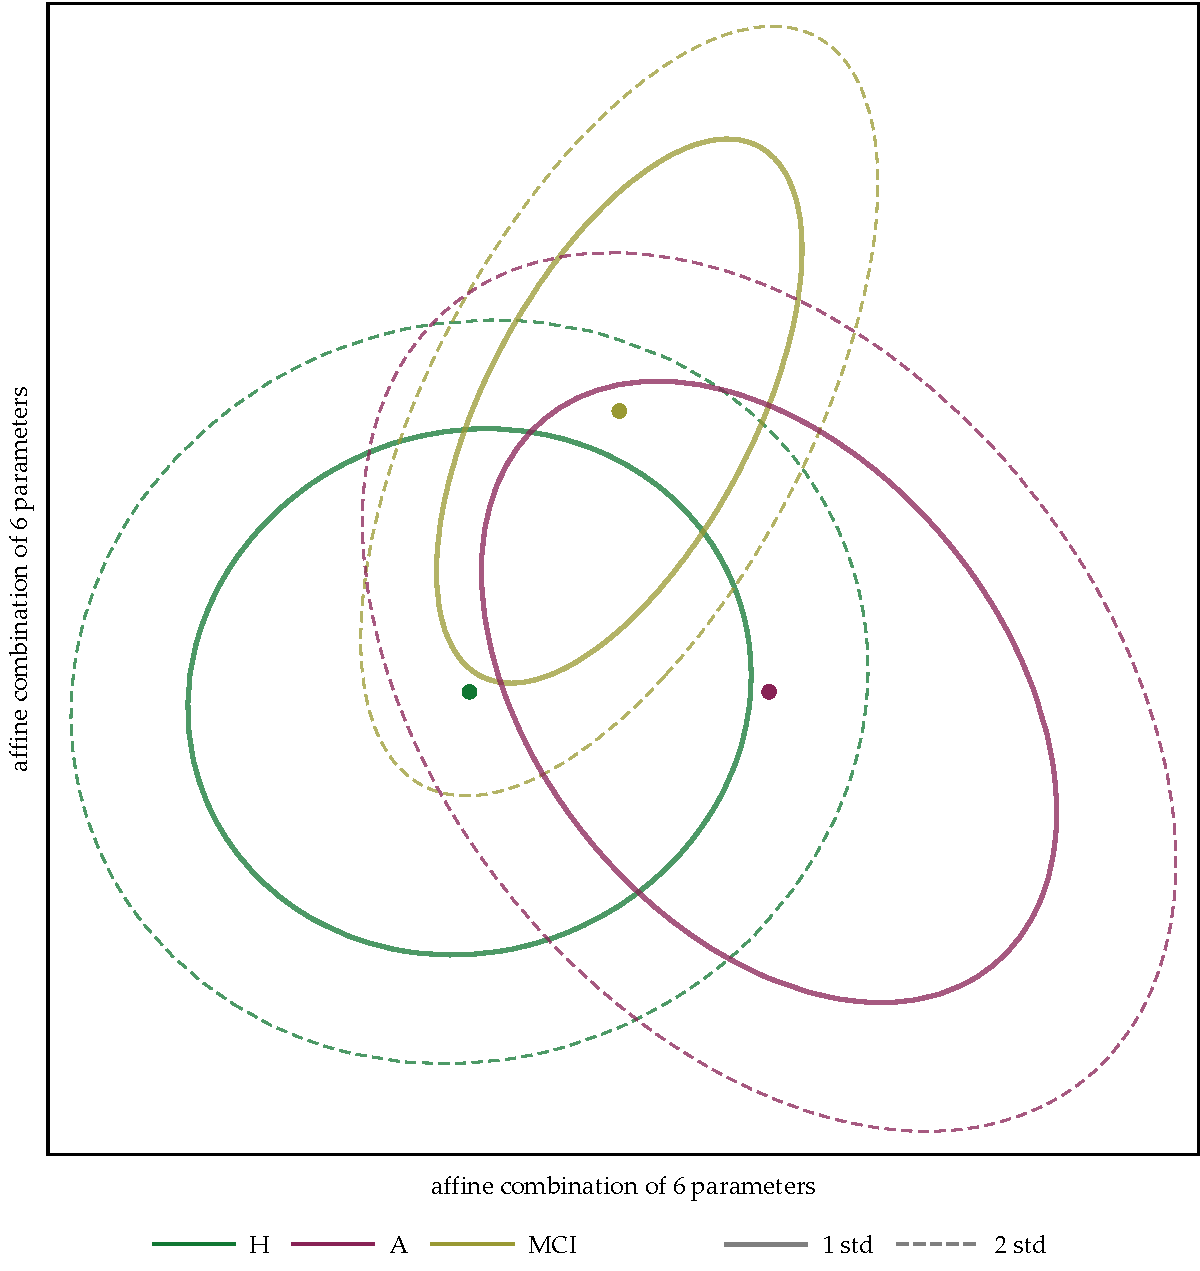
\includegraphics[width=\linewidth]{stds_6_params.pdf}%
\caption{Contours of 1 and 2 standard deviations of the distributions
  $\pf(\yxx \| \text{health condition}, \data)$, on a two-dimensional
  section of the six-dimensional parameter space. The sectioning plane
  passes through the expectations of the three distributions, denoted by
  the dots. The distributions can overlap even more or even less than this
  in the remaining four dimensions.}
\label{results_regions}
\end{figure}

\begin{figure}[!h]
  \centering
\hfill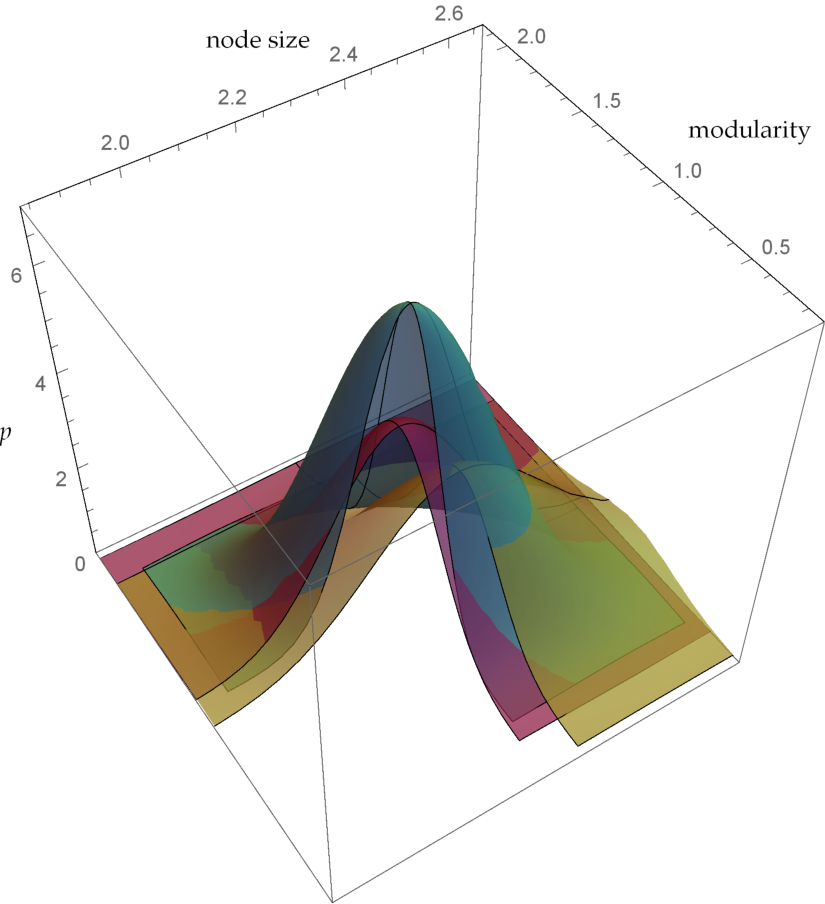
\includegraphics[width=0.3\linewidth]{nodesize_vs_modularity3D.pdf}\\%
\vspace{-0.36\linewidth}  
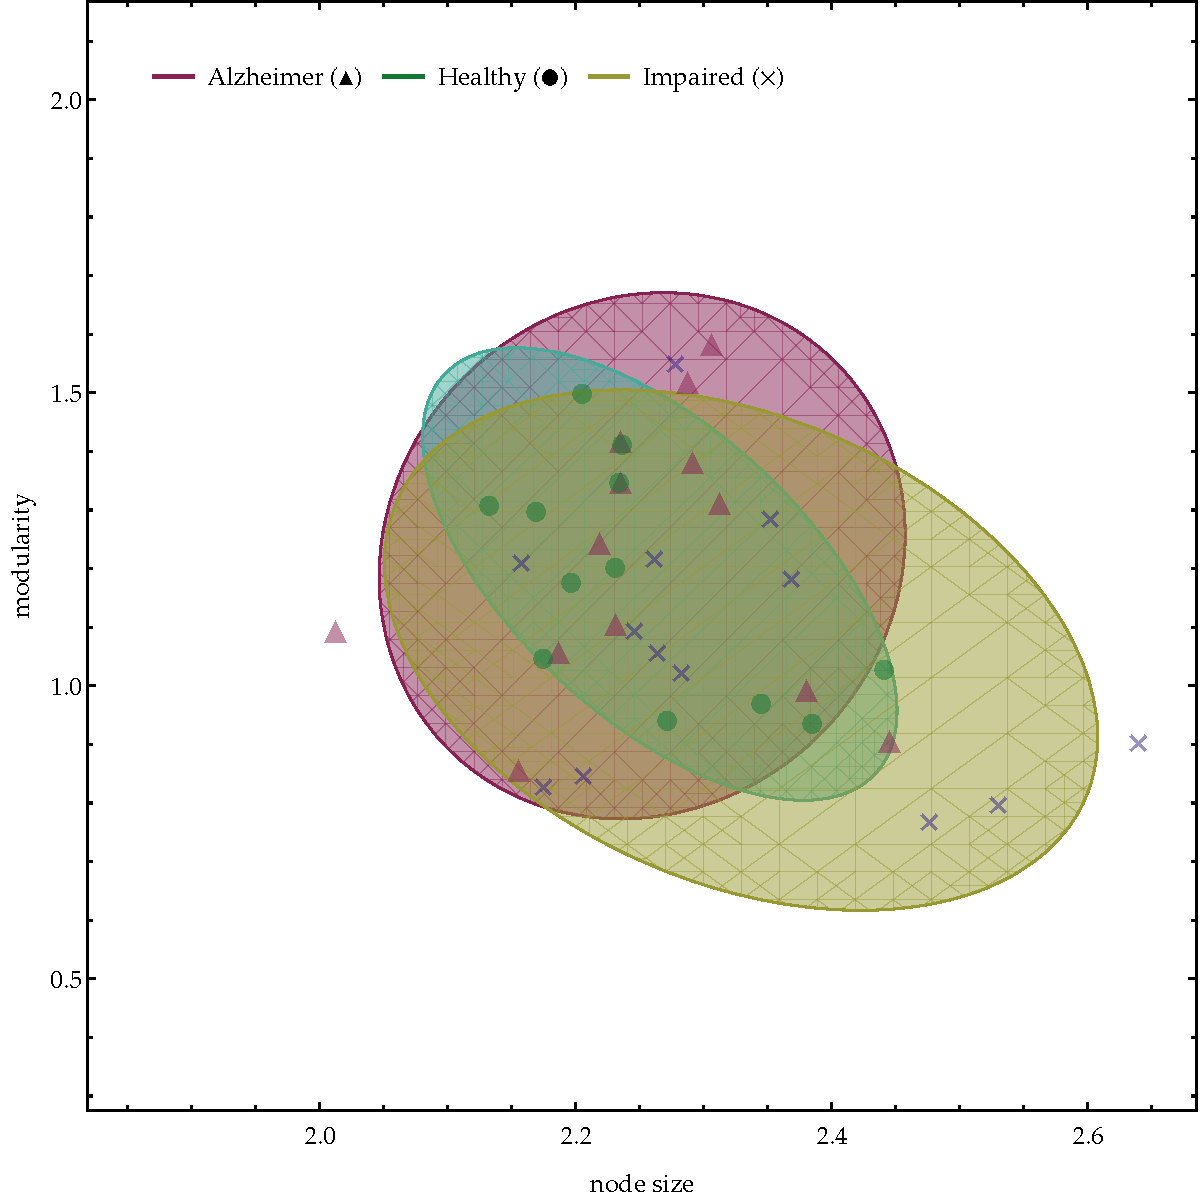
\includegraphics[width=\linewidth]{nodesize_vs_modularity.pdf}%
\caption{Approximate representation of
  $\pf(\yxx \| \text{health condition},
  \data)$. The indicator $\yxx$ is the vector
  $(\text{node size},\text{modularity})$, the health condition is
  Alzheimer, Healthy, or cognitively Impaired. The coloured regions are the
  areas in which the indicator lie with $70\,\%$ probability. Red:
  $\pf(\text{indicator} \| \ya, \data)$, green:
  $\pf(\text{indicator} \|\yh, \data)$, yellow:
  $\pf(\text{indicator} \| \yi, \data)$. The marks represent Simone's
  data, table~\ref{tab:simones_data}. The upper right inset gives a 3D
  idea. See discussion on p.~\pageref{eq:results_discussion} for further
  explanation.}
\label{results_regions_old}
\end{figure}

\clearpage

\section{Final remarks}
\label{sec:remarks}

\subsection{Generalizations}
\label{sec:generalizations}

In this example we have used the known means, variances, and covariances of
the parameters as \enquote{sufficient statistics}. Two generalizations
are immediately clear.

% First, we could use other two parameters, or three or more, obtained from
% the fMRI graph data. The file \texttt{simonedata\_all.pdf} accompanying
% this note, reproduced in miniature as \fig~\ref{results_regions_all_pairs}
% on p.~\pageref{results_regions_all_pairs}, shows a \emph{qualitative} estimate
% (maximum likelihood) of the results for all possible pairs from: average
% degree, average edge weight, clustering coefficient, node size, shortest
% path length, graph size, modularity. The pairs (average degree,
% clustering), (average degree, graph size), (clustering coefficient, graph
% size), (shortest path length, graph size) seem to be promising. One must
% make sure, however, that the graph size really relates to the brain
% configuration, and not to slightly different fMRI scan methods among the
% three health categories.

First, we could use different statistics from the data, for example all
moments up to the third, fourth, or higher. The formulae we obtain in all
these cases are analogous to~\eqref{eq:assumption2probability}; in
particular, we obtain integrals with exponentials of all the included
moments. However, if the number of statistics is comparable to the number
of data then the resulting distributions will appear almost flat. Also, the
more statistics we include, the more dimensions in the integrations to
perform; see the next subsection on this point.

A second generalization is to assume slightly different inferential
relevances. For example, for predicting whether the patient has Alzheimer
we can assume that the health indicators of the individuals with
\emph{every} health condition are relevant -- not only of those with
Alzheimer. Also in this case we obtain formulae uniquely determined by
these assumptions.


% \subsection{Analytic approximations}
% \label{sec:approximations}

% Plot~\ref{results_regions} uses normal approximations of the distributions
% $\pf(\yxx\|\yH,\data)$, but the latter could be more asymmetric and
% have fatter tails than a normal. It is computationally very heavy to plot
% them, however, if we have to perform the integrals in their formulas for
% many values of $\yxx$. A very rough approximation of the integrals is given
% by the maximum value of the integrand, but it does not work well for data
% with few individuals: compare plot~\ref{results_regions} and the
% corresponding plot in the file \texttt{simonedata\_all.pdf} for example.
% Higher-order approximations can be obtained with Moritz's diagrammatic
% methods, as explained in his lecture notes; they are very valuable in case
% of scarce data.


\subsection{Maximum likelihood, Kullback-Leibler, \amp\ co.}
\label{sec:max_likelihood}

Formula~\eqref{eq:assumption2probability} contains, as approximations,
formulae that are used in some literature to solve this same problem.

The multidimensional Student's $t$-distribution is related to the
$\varChi^2$ one. It is well known in statistics: it has fatter tails than
a Gaussian, and this makes it more robust against the presence of outliers;
that is, outliers won't move its peaks away from the bulk of the data, as
it can happen for the Gaussian distribution instead.

An important point, for me, is that this distribution has appeared
automatically from our assumption of p.~\pageref{eq:assumption} and the
rules of probability theory. We have not invoked ad hoc on grounds of
robustness or for other reasons.

If our data has many individuals, the $t$-distribution tends to a Gaussian.
With many individuals, the integral in~\eqref{eq:assumption2probability}
becomes very peaked and we can approximate it with the maximum value of the
integrand. This corresponds to a maximum-likelihood solution and the
classical estimates of the means, variances, covariance of a normal
distribution. In our example this approximate solution is quite bad: it
gives relative errors of 230\,\% for the covariance matrix. Note that
maximum-likelihood also requires that we specify a statistical parametric
model to start with.

The Kullback-Leibler divergence between a \enquote{test distribution} and
the empirical distribution of the data  appears in the exponent of the
integral, if we have numerous individuals. This in turn leads to a
maximum-entropy solution as approximation.


\subsection{Using histograms}
\label{sec:histograms}

Simone wanted to somehow compare the histograms of the distribution of the
parameters obtained from the fMRI, for the different health conditions.
This can be done in the method shown here. The data in the histogram of a
quantity $X$ over $n$ bins are equivalent to the first $n$ moments of this
quantity: $\sum X$, $\sum X^2$, $\sum X^3$, \etc. The use of these $n$
moments as sufficient statistics, in the method shown in this note, is
equivalent to the use of the full histogram. This method would roughly
correspond to a comparison of the histograms by means of their
Kullback-Leibler divergence.

% \begin{figure}[p]
%   \centering  
% \includegraphics[width=\linewidth]{simonedata_all.pdf}%
% \caption{Rough estimates of
%   $\pf(\yxx \| \text{health condition}, \data)$ for all pairs of
%   datasets provided by Simone. See file \texttt{simonedata\_all.pdf} for a
%   more readable graphics.}
% \label{results_regions_all_pairs}
% \end{figure}

%\clearpage
\ifpublic
\begin{acknowledgements}
  PGLPM thanks Mari \amp\ Miri for continuous encouragement and affection,
   Buster Keaton and Saitama for filling life with awe and
  inspiration, and  the developers and maintainers of \LaTeX, Emacs, AUC\TeX,
  Open Science Framework, biorXiv, PhilSci, Hal archives, Python, Inkscape,
  Sci-Hub for making a free and unfiltered scientific exchange possible.
%\rotatebox{15}{P}\rotatebox{5}{I}\rotatebox{-10}{P}\rotatebox{10}{\reflectbox{P}}\rotatebox{-5}{O}.
%\sourceatright{\autanet}
\end{acknowledgements}
\fi

%\appendixpage
%\appendix

%%%%%%%%%%%%%%% BIB %%%%%%%%%%%%%%%

\defbibnote{prenote}{{\footnotesize (\enquote{van $X$} is listed under V;
    similarly for other prefixes, regardless of national
    conventions.)\par}}
% \defbibnote{postnote}{\par\medskip\noindent{\footnotesize% Note:
%     \arxivp \mparcp \philscip \biorxivp}}

\printbibliography[prenote=prenote%,postnote=postnote
]

\end{document}
---------- cut text ----------------


\begin{equation}
  \label{eq:assumption2probability}
\begin{split}
  &\!\begin{multlined}[0.9\linewidth]
    \pf[(\ya,\yxx_0) \| \set{\yH_i,\yxx_i}] ={}\\
    \int \yN(\yxx_0 \| \ymma,\yssa)\,\yfa \,
    \yq(\yfa,\yfh,\yfi,\ymma,\yssa,\ymmh,\yssh,\ymmi,\yssi \|
    \set{\yH_i,\yxx_i})
    \times{}\\
    \,\di\yfa\,\di\yfh\,\di\yfi\,\di\ymma\,\di\yssa\,\di\ymmh\,\di\yssh\,\di\ymmi\,\di\yssi
  \end{multlined}
  \\[2\jot]
  &\!\begin{multlined}[0.9\linewidth]
    \pf[(\yh,\yxx_0) \| \set{\yH_i,\yxx_i}] ={}\\
    \int \yN(\yxx_0 \| \ymmh,\yssh)\,\yfh \,
    \yq(\yfa,\yfh,\yfi,\ymma,\yssa,\ymmh,\yssh,\ymmi,\yssi \|
    \set{\yH_i,\yxx_i})
    \times{}\\
    \,\di\yfa\,\di\yfh\,\di\yfi\,\di\ymma\,\di\yssa\,\di\ymmh\,\di\yssh\,\di\ymmi\,\di\yssi
  \end{multlined}
  \\[2\jot]
  &\!\begin{multlined}[0.9\linewidth]
    \pf[(\yi,\yxx_0) \| \set{\yH_i,\yxx_i}] ={}\\
    \int \yN(\yxx_0 \| \ymmi,\yssi)\,\yfi \,
    \yq(\yfa,\yfh,\yfi,\ymma,\yssa,\ymmh,\yssh,\ymmi,\yssi \|
    \set{\yH_i,\yxx_i})
    \times{}\\
    \,\di\yfa\,\di\yfh\,\di\yfi\,\di\ymma\,\di\yssa\,\di\ymmh\,\di\yssh\,\di\ymmi\,\di\yssi
  \end{multlined}
\end{split}
\end{equation}

\begin{multline}
  \label{eq:params_posterior}
  \yq(\yfa,\yfh,\yfi,\ymma,\yssa,\ymmh,\yssh,\ymmi,\yssi \| \set{\yH_i,\yxx_i})
  \propto{}\\
  \biggl[ \prod_i^{\yH_i=\ya} \yN(\yxx_i \| \ymma,\yssa)\,\yfa \biggr]\,
  \biggl[ \prod_i^{\yH_i=\yh} \yN(\yxx_i \| \ymmh,\yssh)\,\yfh \biggr]\,
  \biggl[ \prod_i^{\yH_i=\yi} \yN(\yxx_i \| \ymmi,\yssi)\,\yfi \biggr]
  \times{}\\
  \yq(\yfa,\yfh,\yfi,\ymma,\yssa,\ymmh,\yssh,\ymmi,\yssi)
\end{multline}

*** simone's old data ***

\begin{table}[!h]
  \centering
  \begin{minipage}[t]{0.3\linewidth}\footnotesize
    \begin{tabular}[t]{@{}c@{\quad}c@{\quad}c@{}}
      $i$ & $\yH_i$ & $\yxx_i$ \\ \midrule
      $1$ & A & $(2.219,1.250)$ \\
      $2$ & A & $(2.306,1.590)$ \\
      $3$ & A & $(2.287,1.524)$ \\
      $4$ & A & $(2.235,1.355)$ \\
      $5$ & A & $(2.231,1.112)$ \\
      $6$ & A & $(2.187,1.064)$ \\
      $7$ & A & $(2.235,1.423)$ \\
      $8$ & A & $(2.155,0.8617)$ \\
      $9$ & A & $(2.313,1.318)$ \\
      $10$ & A & $(2.012,1.099)$ \\
      $11$ & A & $(2.380,0.9982)$ \\
      $12$ & A & $(2.291,1.388)$ \\
      $13$ & A & $(2.445,0.9115)$ 
    \end{tabular}
  \end{minipage}\hfill%
  \begin{minipage}[t]{0.3\linewidth}\footnotesize
    \begin{tabular}[t]{@{}c@{\quad}c@{\quad}c@{}}
      $i$ & $\yH_i$ & $\yxx_i$ \\ \midrule
    $14$    & H & $(2.169,1.301)$ \\
    $15$    & H & $(2.133,1.310)$ \\
    $16$    & H & $(2.234,1.350)$ \\
    $17$    & H & $(2.231,1.205)$ \\
    $18$    & H & $(2.205,1.501)$ \\
    $19$    & H & $(2.345,0.9723)$ \\
    $20$    & H & $(2.236,1.415)$ \\
    $21$    & H & $(2.197,1.180)$ \\
    $22$    & H & $(2.175,1.050)$ \\
    $23$    & H & $(2.385,0.9397)$ \\
    $24$    & H & $(2.272,0.9442)$ \\
    $25$    & H & $(2.441,1.032)$ 
      % $39$ & H & $(0.,0.)$ \\
    \end{tabular}
  \end{minipage}\hfill%
    \begin{minipage}[t]{0.3\linewidth}\footnotesize
    \begin{tabular}[t]{@{}c@{\quad}c@{\quad}c@{}}
      $i$ & $\yH_i$ & $\yxx_i$ \\ \midrule
   $26$  & I & $(2.278,1.551)$ \\
   $27$   & I & $(2.283,1.024)$ \\
   $28$   & I & $(2.263,1.058)$ \\
   $29$   & I & $(2.206,0.8472)$ \\
   $30$   & I & $(2.640,0.9041)$ \\
   $31$   & I & $(2.476,0.7693)$ \\
   $32$   & I & $(2.246,1.094)$ \\
   $33$   & I & $(2.369,1.184)$ \\
   $34$   & I & $(2.157,1.210)$ \\
   $35$   & I & $(2.530,0.7979)$ \\
   $36$   & I & $(2.175,0.8279)$ \\
   $37$   & I & $(2.261,1.218)$ \\
   $38$   & I & $(2.352,1.286)$ 
    \end{tabular}




    \begin{table}[!h]
  \centering\footnotesize
  \begin{minipage}{\linewidth}\footnotesize
    \begin{equation*}
\begin{aligned}
  \yna&=13, & \vxxa&=(2.253, 1.223), & \vxta&=
  \begin{pmatrix}
    0.01050 & 0.001881\\ &0.05003
  \end{pmatrix}
  \\
  \ynh&=12, &\vxxh&=(2.252, 1.183), & \vxth&=
  \begin{pmatrix}
    0.007970 & -0.01015 \\ &0.03459
  \end{pmatrix}
  \\
  \yni&=13, &
  \vxxi&=(2.326, 1.059),&  \vxti&=
  \begin{pmatrix}
    0.01921 & -0.01036 \\ &0.04875
  \end{pmatrix}
\end{aligned}
%\label{eq:simone_suff_stat}
\end{equation*}
  \end{minipage}
  \caption{Simone's data, with
    $\yxx_i=(\text{node size},\text{modularity})$, and their statistics
    used by our assumption. Node size has been divided by $10$ and
    modularity multiplied by $10$ to have numbers of order unity. Rounding
    is to four significant figures.}
  \label{tab:simones_data}
\end{table}


\clearpage
\begin{table}[!ht]
  \centering%\footnotesize
  \begin{tabular}[t]{@{}l@{\quad}c@{\quad}c@{\quad}c@{}}
  &  $\pf(\yxx\|\ya,\data)$ &
    $\pf(\yxx\|\yh,\data)$ &
    $\pf(\yxx\|\yi,\data)$ \\ \midrule
expectations  & $(2.25,1.22)$   & $(2.27,1.19)$     & $(2.33,1.06)$    \\
variances & $(0.0192,0.0917)$   & $(0.0156,0.0679)$ & $(0.0354,0.0898)$\\
covariance & $0.00344$          & $-0.0197$         & $-0.0189$        
  \end{tabular}
  \caption{Main moments $\expe{\yxx}$, $\expe{\yxx\T\yxx}$ of the
    distributions $\pf(\yxx \| \text{health condition}, \data)$, with
    $\yxx=(\text{node size},
    \text{modularity})$.}\label{tab:features_results}
\end{table}


%%% Local Variables: 
%%% mode: LaTeX
%%% TeX-PDF-mode: t
%%% TeX-master: t
%%% End: 
